% Compile with: latexmk -pdf paper.tex (from docs/paper, where refs.bib, figs/ and the ICML style files live).
% ICML 2026 style (icml/icml2026.zip). Submission mode hides the authors; use \usepackage[accepted]{icml2026} for the camera-ready.
\documentclass{article}
\usepackage{microtype}
\usepackage{graphicx}
\usepackage{booktabs}
\usepackage{hyperref}
\usepackage{icml2026}
\usepackage{amsmath,amssymb,amsthm}
\usepackage{needspace}

\newtheorem{theorem}{Theorem}
\newtheorem{proposition}[theorem]{Proposition}
\newtheorem{corollary}[theorem]{Corollary}
\newtheorem{definition}{Definition}
\newtheorem{lemma}{Lemma}[section]
\newcommand{\ess}{\mathrm{ESS}}
\newcommand{\E}{\mathbb{E}}
\newcommand{\R}{\mathbb{R}}

\icmltitlerunning{A Description Is Likely Not Worth a Thousand Demonstrations}

\begin{document}

\twocolumn[
\icmltitle{A Description Is Likely Not Worth a Thousand Demonstrations: \\ Measuring the Effective Sample Size of Task Descriptions in In-Context Learning}
\begin{icmlauthorlist}
\icmlauthor{Bruce Quan Nguyen}{dec,ua}
\end{icmlauthorlist}
\icmlaffiliation{dec}{Decaude Labs}
\icmlaffiliation{ua}{University of Alberta, Edmonton, Canada}
\icmlcorrespondingauthor{Bruce Quan Nguyen}{bruce.nguyen@decaude.com, trungqua@ualberta.ca}
\icmlkeywords{in-context learning, task description, effective sample size, Bayesian inference}
\vskip 0.3in
]
\printAffiliationsAndNotice{}

\begin{abstract}
Prompts for in-context learning usually combine a task description with demonstrations, yet theories of in-context learning mostly model only the demonstrations. We ask how many demonstrations a description is worth. We define the \emph{effective sample size} (ESS) of a description as the number of demonstrations that lower a Bayes-optimal predictor's regret by the same amount, and study it in in-context linear regression. The ESS is set by the description's \emph{specificity}, how much uncertainty about the task it removes, and its \emph{reliability}, the probability that it is relevant. For a reliable description, we prove that the ESS grows linearly in the task dimension when the description is loose and in inverse proportion to the variance it leaves when it is specific. For a description that may be irrelevant, the ESS without demonstrations stays bounded however specific the description is, and a predictor that trusts it fully can do worse than one that ignores it. Meta-trained Transformers come close to the Bayes-optimal ESS for reliable descriptions and inherit their trust in a description from their training distribution. Pretrained language models told a description's specificity and reliability in words use the description, and gain more from a more specific one, but a description with a Bayes-optimal ESS of thirty-six has an ESS of at most eight for them, because they rely on it by a fixed amount that neither its stated specificity nor its stated reliability moves.
\end{abstract}

\section{Introduction}
\begin{figure*}[t]
\centering
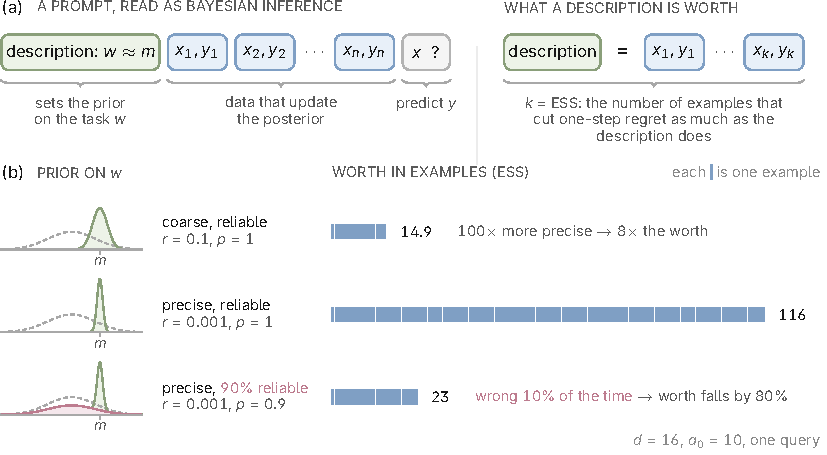
\includegraphics[width=5.5in]{figs/overview.pdf}
\caption{\textbf{A description is worth a number of demonstrations, set by how much it narrows the task and how likely it is to be about the task.} (a) A prompt read as Bayesian inference, and the ESS of its description. (b) The prior on the task given three descriptions (sketched, not to scale), and the ESS of each with no demonstrations in hand, at $d = 16$ and $a_0 = 10$. Specificity raises the ESS (\S\ref{sec:specificity}); a one-in-ten chance of being unrelated to the task removes most of that gain (\S\ref{sec:reliability}).}
\label{fig:overview}
\end{figure*}
A prompt for in-context learning (ICL) usually carries two kinds of information about the task: a description in natural language and a few demonstrations \citep{brown2020}. In practice the description is an instruction; we read it as a statement about the task, since its value lies in what it says the task is, and set aside how a model is made to follow it. The evidence on what a description contributes is mixed. In prompt-based fine-tuning a well-crafted prompt can be worth hundreds of data points \citep{lescao2021}, and a written summary can stand in for many demonstrations \citep{honda2025}, yet models also perform adequately with misleading descriptions \citep{webson2022} and can prioritize demonstrations over explicit instructions \citep{gupta2025}. Theories of ICL mostly model the prompt as a sequence of demonstrations \citep{garg2022, akyurek2023, xie2022}. Those that add a description show that a learner can use it to predict better \citep{huangge2025}, but not how much it is worth in the unit a prompt writer trades it against: demonstrations. We ask the question directly: how many demonstrations is a task description worth, and what determines the number? Our title answers for descriptions as they come: a reliable and very specific description can be worth thousands (Theorem~\ref{prop:reliable}), but one that may be irrelevant is worth a bounded number however specific it is (Corollary~\ref{cor:ess}), and the pretrained models we test treat even a specific one as worth a few.

We take the Bayesian view of ICL \citep{xie2022}. Pretraining gives the model a prior over a latent task, and the prompt is evidence about that task. A demonstration is one noisy observation of the task's input-output behaviour. A description is a statement about the task itself, and conditioning on it gives a sharper prior. Bayesian statistics measures the information in a prior by its effective sample size (ESS), the number of observations that would carry the same information \citep{morita2008}. We define the ESS of a description in the same way and compute it in noisy in-context linear regression with a Gaussian task prior \citep{garg2022, akyurek2023, raventos2023}, where Bayes-optimal prediction has a closed form.

Two properties of a description determine its ESS. The first is its \emph{specificity}: a description may state exactly how to do the task or only loosely indicate it, and the more specific it is, the less uncertainty about the task it leaves. The second is its \emph{reliability}: the probability that it is relevant, since a description can conflict with the task the demonstrations come from \citep{evans2006}. Our contributions are:
\begin{itemize}
    \item \textbf{A common unit.} We define the ESS of a task description as the number of demonstrations that lower a Bayes-optimal predictor's regret by the same amount (Definition~\ref{def:ess}). It puts descriptions and demonstrations on one scale, and it can be measured for any learner from its answers alone.
    \item \textbf{What specificity is worth.} For a reliable description, we prove that the ESS grows linearly in the task dimension $d$ when the description is loose and linearly in $1/r$ when it is specific, where $r$ is the fraction of the prior variance the description leaves (Theorem~\ref{prop:reliable}). Roughly, it is $(d-1)(1-r) + 1/(r a_0)$.
    \item \textbf{What unreliability costs.} For a description that is relevant with probability $p$, the regret is that of a predictor told whether the description is relevant, plus the information the next label carries about relevance, which totals at most the entropy $H(p)$ over the whole prompt (Proposition~\ref{prop:unreliable}). Consequently, the ESS without demonstrations is bounded however specific the description is, and with many demonstrations it is at most $p$ times that of a reliable description (Corollary~\ref{cor:ess}). A predictor that instead trusts the description fully pays a penalty that grows with specificity, and a specific description that is sometimes irrelevant can then be worse than none.
\end{itemize}
We then measure the ESS in two kinds of learner. Meta-trained Transformers come close to the Bayes-optimal ESS for reliable descriptions, and their trust in a description follows the reliability they were trained on (\S\ref{sec:networks}). Pretrained language models, told a description's specificity and reliability in words, use the description but rely on it by a fixed amount, so a description with a Bayes-optimal ESS of thirty-six has an ESS of a few for them (\S\ref{sec:llm}).

\section{Related Work}
\paragraph{ICL as Bayesian inference.} Our approach builds on the understanding of ICL as implicit Bayesian inference \citep{xie2022}, in which meta-trained Transformers have been shown to implement optimal estimators such as Bayes-optimal ridge regression \citep{akyurek2023, raventos2023, panwar2024}.

\paragraph{Task descriptions in theories of ICL.} Some of this literature includes task descriptions, modeling them as tokens that indicate hypothesis classes or carry input means \citep{huangge2025, lin2025, tong2026, lin2024}, but these works generally do not quantify the description's value in units of examples, nor do they formalize the probability that a description is irrelevant. Closest to our setting, \citet{zhu2026} show that a Transformer given a prefix of related datasets performs amortised hierarchical Bayesian prediction; we express the value of such conditioning information in demonstrations and allow it to be irrelevant.

\paragraph{Effective sample size of a prior.} Our ESS follows the prior sample size methods of Bayesian statistics \citep{morita2008, reimherr2021, neuenschwander2020}, particularly those that use predictive regret \citep{reznik2026}. To model a description that may be irrelevant we use a robust mixture prior, a technique from clinical trials for historical data that may conflict with the trial \citep{schmidli2014}.

\paragraph{Descriptions and priors in pretrained language models.} Empirical work has priced prompts in training examples: \citet{lescao2021} in prompt-based fine-tuning, and \citet{cook2026}, who find that one instruction in fine-tuning data can stand in for up to a hundred execution examples. \citet{wenliang2025} treat a prompt as conditioning for a Bayesian sequence predictor and find that an optimized prompt can be shorter than demonstrations of equal effect. Tests of pretrained models against a known optimum on synthetic tasks find that in-context evidence outweighs a stated prior \citep{gupta2025}, that learning curves approach a Bayesian reference \citep{akata2026}, and that models estimate a density from numbers in context like a kernel estimator of adaptive width \citep{liu2025}. We add to such a test a description of stated specificity and stated reliability, and measure its ESS against the Bayes-optimal ESS.

\section{Problem Setup}\label{sec:setting}

\paragraph{Tasks and demonstrations.}
Think of a task as a hidden weight vector $w \in \R^d$. A demonstration is a random input $x \sim \mathcal{N}(0, I_d)$ paired with its output label $y \sim \mathcal{N}(w^\top x, 1)$: the label is $w^\top x$ plus Gaussian noise, and we measure labels in units of that noise, so the noise variance is $1$. We start with a broad ``base prior'' belief that the weights are centered around zero, $w \sim \mathcal{N}(0, a_0 I_d)$. Since the noise variance is $1$, the prior variance $a_0$ is also the signal-to-noise ratio. The numerical results use $a_0 = 10$.

\paragraph{Descriptions.}
A description is a suggested weight vector $m \in \R^d$, drawn as $m \sim \mathcal{N}(0, (1-r)\,a_0 I_d)$. However, descriptions aren't always helpful. We use a hidden coin flip $Z \sim \mathrm{Bernoulli}(p)$, independent of $m$, to decide if the description is \emph{relevant} ($Z=1$) or \emph{irrelevant} ($Z=0$).
\begin{itemize}
    \item \textbf{If relevant:} The true weights are clustered around the suggested vector, $w \mid m \sim \mathcal{N}(m, r a_0 I_d)$: in every direction the variance drops to a fraction $r$ of the base variance.
    \item \textbf{If irrelevant:} The true weights ignore the description, $w \sim \mathcal{N}(0, a_0 I_d)$ independently of $m$. The description tells us nothing useful.
\end{itemize}
Either way, $w$ marginally has the base prior, and $m$ has the same distribution, so seeing $m$ alone says nothing about whether it is relevant. Averaging over $Z$, the prior for $w$ given $m$ is the robust mixture $p\,\mathcal{N}(m, r a_0 I_d) + (1-p)\,\mathcal{N}(0, a_0 I_d)$ \citep{schmidli2014}. Here, the parameter $r \in (0,1)$ measures the description's \textbf{specificity}: $r$ near $1$ means it's a very vague hint, while $r$ near $0$ means the description practically gives away the exact answer. The probability $p$ measures the description's \textbf{reliability}. If $p=1$, the description is always relevant, and we call it \emph{reliable}.

\paragraph{Regret and ESS.}
A predictor sees a prompt $D$ (the description, $n$ demonstrations, and a query input $x$) and gives a predictive density $f(y \mid D)$ for the query's label. To measure how well it does, we look at its ``predictive regret'': the expected penalty (in log loss) it pays compared to an oracle that perfectly knows the true weights $w$, the per-step regret of \citet{genewein2025}:
\begin{equation}\label{eq:regret}
    R = \E \left[ -\log f(y \mid D) + \log \phi(y; w^\top x, 1) \right],
\end{equation}
where $\phi$ is the Gaussian density. Let $R^{\mathrm{ex}}(n)$ be the regret of the Bayes-optimal predictor that relies strictly on $n$ demonstrations, $R^{\mathrm{desc}}(n)$ that of the Bayes-optimal predictor that also has the description, and $R^{\mathrm{desc}}_{p=1}(n)$ the value of $R^{\mathrm{desc}}(n)$ for a reliable description.
\begin{definition}[Effective Sample Size]\label{def:ess}
The Effective Sample Size (ESS) measures how many demonstrations a description is worth. If we currently have $n$ demonstrations and a description, the ESS is the number of additional demonstrations $\ess_n$ we would need to achieve the same regret without the description. Mathematically, it is $\ess_n = n^* - n$, where $n^* \ge 0$ is the smallest solution of $R^{\mathrm{ex}}(n^*) = R^{\mathrm{desc}}(n)$ (interpolating the baseline regret curve linearly between integers). If the regret with the description is above the regret with nothing at all, we write $\ess_n \le -n$. The standalone ESS ($n=0$) is written $\ess_0$, or simply $\ess$.
\end{definition}
It belongs to a kind of description, set by $r$ and $p$, not to one particular $m$, and it is the data-dependent prior sample size of \citet{reimherr2021} with predictive regret as the measure of uncertainty. For the Bayes-optimal predictor it is never negative: knowing the description can never raise its expected log loss, so $R^{\mathrm{desc}}(n) \le R^{\mathrm{ex}}(n)$, and the baseline regret only falls as demonstrations arrive. The same definition applies to any other learner through its own two regret curves; there it is negative when the description hurts.

\section{Specificity: Reliable Descriptions}\label{sec:specificity}
A reliable description narrows the prior over the task; Theorem~\ref{prop:reliable} counts the demonstrations that would narrow it as much. With a reliable description ($p = 1$) the posterior over $w$ is Gaussian with some covariance $\Sigma$, and the regret is half the expected log of the predictive variance relative to the noise, $R = \tfrac12 \E \log(1 + x^\top \Sigma x)$.

\needspace{10\baselineskip}
\begin{theorem}[Effective Sample Size of a Reliable Description]\label{prop:reliable}
Suppose our description is always relevant ($p = 1$). Let $c = 1 / (r a_0)$, the noise variance over the description's prior variance (its conjugate-prior ESS). The description's value $\ess$ falls into two regimes:
\begin{enumerate}
    \item[(i)] \textbf{Loose descriptions:} If the description is vague ($c \le 1$), it is worth roughly $d(1-r)$ demonstrations. More precisely, as $rd \to \infty$, $\ess = (d-1)(1-r) + (1-r)c + O(1/(rd))$.
    \item[(ii)] \textbf{Specific descriptions:} If $a_0 \ge 1$ and the description is very specific ($c$ much larger than $d$), it is worth roughly $c + d$ demonstrations. More precisely, as $c/d \to \infty$, $\ess = c + d + 1 - 1/a_0 + O(d/c)$.
    \item[(iii)] \textbf{Hard bound:} No matter the parameters, the description can never be worth more than $c + d + 2$ demonstrations.
\end{enumerate}
\end{theorem}
Appendix~\ref{app:specificity} states the theorem in a fuller form and proves it. In both regimes the ESS is the sum of two terms. The first counts dimensions: about $(1-r)(d-1)$ demonstrations for a loose description and $d+1$ for a specific one, because at high signal-to-noise ratio each of the first $d$ demonstrations removes the uncertainty in one direction. The second is the conjugate-prior ESS $c$, the number of unit-noise observations of $w$ that carry as much information as a prior of variance $r a_0$ \citep{neuenschwander2020}, of which the base prior already supplies $1/a_0$. A single formula summarizes both regimes: $\ess \approx (d-1)(1-r) + 1/(ra_0)$. It differs from the expansion in (i) by $1/a_0$ and from the one in (ii) by under two demonstrations. Between the regimes only the bound (iii) applies, but at every $r$ in Figure~\ref{fig:ess}a the formula is within two demonstrations of the exact ESS. At $d = 16$ and $a_0 = 10$, a description that leaves a tenth of the prior variance ($r = 0.1$) is worth $14.9$ demonstrations, and one that leaves a thousandth ($r = 0.001$) is worth $117$ (Figure~\ref{fig:ess}a). With many demonstrations in hand the dimension term fades, since the demonstrations have already removed that uncertainty (Corollary~\ref{cor:ess}): at $r = 0.1$ the ESS falls from $14.9$ alone to $1.1$ with $100$ demonstrations in hand.

\begin{figure*}[t]
\centering
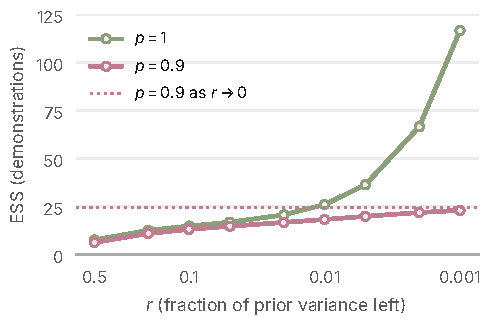
\includegraphics[width=5.5in]{figs/ess.pdf}
\caption{\textbf{Specificity raises the ESS without bound when the description is reliable, and only up to a cap when it may be irrelevant.} ESS of a description against $r$, the fraction of the prior variance it leaves, with $n$ demonstrations in hand ($\ess_n$ of Definition~\ref{def:ess}); one panel per reliability $p$. The ESS of a reliable description grows without bound as it becomes more specific (a). When the description may be irrelevant, the ESS with no demonstrations is capped at the dotted limit, and many demonstrations in hand lift it (b, c). $d = 16$, $a_0 = 10$, eight batches of 8{,}000 prompts, with standard errors below $0.1$ demonstrations ($0.2$ for the dotted line at $p = 0.99$). Dotted: the limit of the standalone ESS as $r \to 0$.}
\label{fig:ess}
\end{figure*}

\section{Reliability: Descriptions That May Be Irrelevant}\label{sec:reliability}
Not knowing whether a description is relevant has a price; the proposition gives it in nats and bounds it. When $p < 1$ the Bayes-optimal predictive is a mixture of two predictives, one that takes the description as relevant and one that ignores it, weighted by the posterior probability that the description is relevant.

\begin{proposition}[Regret of an Unreliable Description]\label{prop:unreliable}
Let $D_n$ be the prompt with $n$ demonstrations and $y$ the label of its query. When a description is relevant only with probability $p$, our predictive regret is the regret of a predictor that is told whether the description is relevant, plus a penalty for not being told:
\begin{equation}\label{eq:decomp}
    R^{\mathrm{desc}}(n) \;=\; p\, R^{\mathrm{desc}}_{p=1}(n) + (1-p)\, R^{\mathrm{ex}}(n) + I_n .
\end{equation}
Here, $R^{\mathrm{desc}}_{p=1}(n)$ is the regret if the description is reliable, $R^{\mathrm{ex}}(n)$ is the baseline regret if we ignore the description completely, and $I_n = I(Z;\, y \mid D_n)$ is the mutual information between the description's relevance $Z$ and the new label given the prompt. Each label resolves part of our uncertainty about $Z$: $I_n = H(Z \mid D_n) - H(Z \mid D_{n+1})$, so $0 \le I_n \le H(p)$, and the penalties summed over all future predictions are at most our initial uncertainty, $\sum_{n \ge 0} I_n \le H(p)$, the binary entropy in nats.
\end{proposition}
Appendix~\ref{app:reliability} gives the proof. The first two terms are the regret of a predictor that is told whether the description is relevant: with probability $p$ it holds a reliable description, and with probability $1-p$ it holds only the demonstrations. So a description that may be irrelevant is worth what a reliable one is worth when it is relevant and nothing when it is not.

The last term is the price of not being told, and under log loss it is exactly what the label reveals about relevance. It depends on the setting, through $d$, $a_0$, $r$, and $n$: it vanishes when the two predictives agree, so that the label says nothing about relevance, and it is largest when a specific description makes them differ sharply ($0.04$ nats at $r = 0.5$ and $0.26$ at $r = 0.001$, with no demonstrations at $d = 16$, $a_0 = 10$, $p = 0.9$). But there are only $H(p)$ nats to learn about $Z$, so the price summed over the whole prompt is at most $H(p)$, whatever $d$, $a_0$, and $r$: $0.33$ nats at $p = 0.9$. This is an average over relevant and irrelevant descriptions. Case by case, the price summed over the whole prompt is at most $\log(1/p)$ when the description is relevant and $\log(1/(1-p))$ when it is irrelevant, $0.11$ and $2.3$ nats at $p = 0.9$, because the mixture starts with weight $p$ or $1-p$ on the right predictive; the irrelevant case is costly but rare. The decomposition is the standard one for a mixture forecaster under log loss \citep{cesabianchi2006, merhav1998}; what is new is what it implies for the ESS.

\needspace{14\baselineskip}
\begin{corollary}[Effective Sample Size of an Unreliable Description]\label{cor:ess}
When a description might be irrelevant, its value depends on how much data we have:
\begin{enumerate}
    \item[(i)] \textbf{Hard cap with no demonstrations:} If $p < 1$, then before seeing any data, the description's value $\ess_0$ cannot exceed a fixed limit $n^*_p$, regardless of how specific the description is (i.e., this bound is independent of $r$). This limit $n^*_p$ is the number of demonstrations needed to drop the baseline regret down to $(1-p)R^{\mathrm{ex}}(0)$; it depends on $d$, $a_0$, and $p$.
    \item[(ii)] \textbf{Discount with many demonstrations:} As we gather abundant data ($n \to \infty$), a reliable description's value $\ess_n$ approaches $c - 1/a_0$. If it is relevant only with probability $p < 1$, it is ultimately worth at most $p$ times as much: $\limsup_{n \to \infty} \ess_n \le p\,(c - 1/a_0)$.
\end{enumerate}
\end{corollary}

\paragraph{Without demonstrations the ESS is bounded.} The average regret cannot fall below the share contributed by irrelevant descriptions, $(1-p)R^{\mathrm{ex}}(0)$, however specific the description is, and (i) turns that floor into a bound on the ESS. At $d = 16$, $a_0 = 10$, and $p = 0.9$ the bound $n^*_p$ is $40$ demonstrations. It applies even to the predictor told whether the description is relevant, so it comes from irrelevant descriptions being worth nothing, not from doubt; not being told lowers the limit of the exact ESS as $r \to 0$ to $25$ (dotted in Figure~\ref{fig:ess}c). Refining $r$ from $0.1$ to $0.001$ raises the ESS of a reliable description from $14.9$ to $117$, but that of a $p = 0.9$ description only from $13.1$ to $23.0$.

\paragraph{In the limit of many demonstrations, the ESS is at most $p$ times the reliable one.} Demonstrations shrink the regret in the irrelevant case, $R^{\mathrm{ex}}(n)$, and so lift the bound. In the limit a reliable description is worth $c - 1/a_0$ demonstrations: the dimension term is gone and what remains is the information the description adds to the base prior. A description that may be irrelevant is then worth at most $p$ times as much. With $100$ demonstrations in hand, the $r = 0.001$ description is worth $109$ demonstrations if reliable and $87.4$ at $p = 0.9$ (Figure~\ref{fig:ess}), against limits of $99.9$ and at most $89.9$.

\paragraph{Full trust.} The Bayes-optimal predictor hedges, and Proposition~\ref{prop:unreliable} prices the hedge at no more than $H(p)$ nats over the whole prompt, on average. A predictor that instead treats the description as certainly relevant predicts as if $p = 1$ whether or not the description is relevant. With no demonstrations its regret is
\begin{equation}\label{eq:trust}
    \begin{split}
    R^{\mathrm{trust}}(0) = {}& R^{\mathrm{desc}}_{p=1}(0) \\
    &+ (1-p)(1-r)\,\E\!\left[\frac{a_0\|x\|^2}{1 + r a_0 \|x\|^2}\right]
    \end{split}
\end{equation}
(Appendix~\ref{app:trust}): the regret of a reliable description plus a penalty for the irrelevant case. The penalty grows as the description becomes more specific, up to $(1-p)\,a_0 d$ as $r \to 0$, and $H(p)$ does not limit it. When the penalty exceeds what the description gains, full trust is worse than ignoring the description. At $d = 16$, $a_0 = 10$, and $p = 0.9$, the $r = 0.001$ description costs the fully trusting predictor $13.7$ nats, against $2.51$ with no description; at $p = 0.99$ the same description costs it $1.43$ nats and still helps.

\section{Meta-Trained Transformers}\label{sec:networks}
The Bayes-optimal predictor knows how specific and how reliable descriptions are. A network can learn both from the distribution it is trained on. We therefore meta-train Transformers on the setting of \S\ref{sec:setting} and ask how close they come to the Bayes-optimal ESS, and where their trust in a description comes from.

\paragraph{Setup.} Prompts use the prefix embedding of \citet{huangge2025}: an optional description token carrying $m$, up to $20$ demonstration tokens, and a query token. The architecture and optimiser follow \citet{garg2022}, at $d = 5$ and $a_0 = 10$; the network outputs a mean and a log variance for the query's label and is trained with log loss, so its regret is on the scale of~\eqref{eq:regret}. The description is omitted in half the training prompts, and the description token supplies only $m$, so each network must learn $r$ and $p$ from its training distribution. We train one network for each combination of a specific ($r = 0.01$) or loose ($r = 0.1$) description with reliability $p \in \{1, 0.99, 0.9\}$, with a second seed at $p = 0.9$, $r = 0.01$, and evaluate each on $20{,}000$ fresh prompts at every $n$ from $0$ to $20$, with and without a description, at all three reliabilities (details in Appendix~\ref{app:networks}). A network's ESS follows Definition~\ref{def:ess} with its own regret curves. We compare it with the Bayes-optimal predictor that uses the reliability the network was trained on (\emph{trained}) and the one that uses the reliability of the test prompts (\emph{calibrated}) (Figure~\ref{fig:networks}; Table~\ref{tab:networks} in Appendix~\ref{app:networks}). A learner's \emph{implied trust} is the weight $q$ for which the predictor that uses the mixture prior of \S\ref{sec:setting} with $q$ in place of $p$ best matches the learner's mean predictions.

\begin{figure*}[t]
\centering
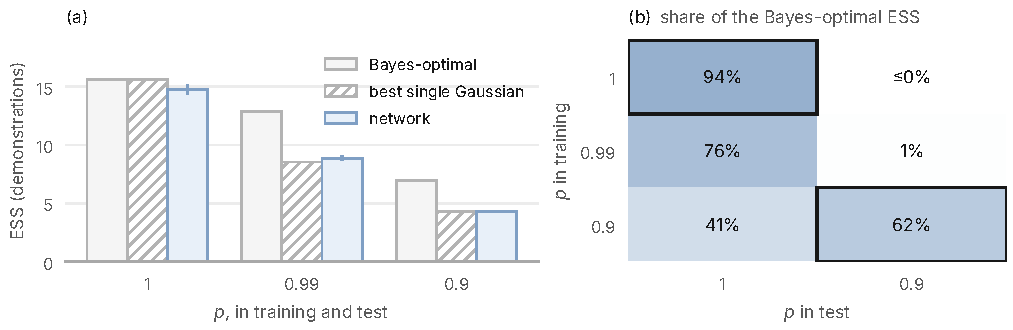
\includegraphics[width=5.5in]{figs/networks.pdf}
\caption{\textbf{Networks reach the Bayes-optimal ESS within what their output can express, and take their trust from training.} ESS with no demonstrations, $d = 5$, $a_0 = 10$; error bars, standard errors over $20{,}000$ prompts. (a) Each network tested at the reliability it was trained on, beside the Bayes-optimal ESS and that of the best single Gaussian: at $p = 1$ the networks match the Bayes-optimal ESS, and below it they match the single-Gaussian limit of their output. (b) The networks trained on specific descriptions ($r = 0.01$) tested at every reliability (the $p = 0.9$ network is the second seed, tested at all three): a network's ESS follows the reliability it was trained on, so the one trained on reliable descriptions loses the description's whole value when one in ten is irrelevant, and the one trained at $p = 0.9$ keeps hedging when all are relevant. Table~\ref{tab:networks} (Appendix~\ref{app:networks}) has every value.}
\label{fig:networks}
\end{figure*}

\paragraph{Networks approach the Bayes-optimal ESS within what their output can express.} Trained and tested on reliable descriptions, the networks come close to the Bayes-optimal ESS: $14.7 \pm 0.4$ against $15.6$ for the specific description, $5.24 \pm 0.05$ against $5.25$ for the loose one (Figure~\ref{fig:networks}a). With descriptions that may be irrelevant and no demonstrations, they fall short of it, to $4.30 \pm 0.07$ against $6.92$ at $p = 0.9$, $r = 0.01$. The cause is the output: the Bayes-optimal predictive is then a mixture of two Gaussians, which a network that emits one mean and one variance cannot express, and the networks match the best single Gaussian instead ($4.29$ in that case). As demonstrations settle whether the description is relevant, the mixture collapses to one component and the networks rejoin the Bayes-optimal predictor: with ten demonstrations in hand that network's ESS is $8.1$ against $9.0$. A second seed reproduces the first, and a network continued to twice the training steps kept the shortfall, so it is not under-training (Table~\ref{tab:networks}).

\paragraph{Trust is inherited from training.} A network's implied trust follows the reliability it was trained on. Networks trained only on reliable descriptions ($p = 1$) have an implied trust near $1$ and behave as the fully trusting predictor of \S\ref{sec:reliability}. When one description in ten is irrelevant, the network trained on specific descriptions has a regret of $2.87$ nats with the description alone against $1.87$ without it ($3.23$ for the fully trusting predictor by~\eqref{eq:trust}, which the network beats by hedging slightly, at an implied trust of $0.999$), so its ESS is at most zero where the calibrated predictor obtains $6.9$. Networks trained at $p = 0.99$ have an implied trust of $0.95$ and lose the specific description's entire value when one in ten is irrelevant ($0.1 \pm 0.4$ against $6.9$). Networks trained at $p = 0.9$ keep hedging, with an implied trust of $0.85$ to $0.9$ across the two seeds, even on prompts whose descriptions are all relevant, where their ESS is $6.4$ and $6.6$ against the calibrated $15.6$ at $r = 0.01$.

\section{Pretrained Language Models}\label{sec:llm}
The networks of \S\ref{sec:networks} know how specific and how reliable descriptions are because they were trained on the task distribution. A pretrained language model has had no such training, and the only way to give it what the Bayes-optimal predictor knows is to say it in the prompt. We say nearly all of it, state a description's specificity and reliability in words, and measure the description's ESS for the model against its Bayes-optimal ESS. The design follows earlier tests of pretrained models against a known optimum on synthetic tasks \citep{gupta2025, akata2026}.

\paragraph{Setting.} We use the simplest case of \S\ref{sec:setting}: one weight ($d = 1$) and the input fixed at $x = 1$, so that a task is a hidden mean $w \sim \mathcal{N}(500, 100^2)$ and a demonstration is a number $y \sim \mathcal{N}(w, \sigma^2)$, rounded to an integer. With inputs the model would also have to do arithmetic; with a single mean, the test is about weighing alone. A description states a value $m$ and a standard deviation $\tau$, and the tasks are drawn so that $w \mid m \sim \mathcal{N}(m, \tau^2)$, the description of \S\ref{sec:setting} with $r = \tau^2 / 100^2$. The Bayes-optimal yardstick knows only what the prompt says: the noise $\sigma$, the description, and otherwise a mean that is unknown, which we take as uniform over the three-digit range. A relevant description then adds the information of $c = \sigma^2 / \tau^2$ demonstrations: the Bayes-optimal squared error is $\sigma^2/(c+n)$ with it and $\sigma^2/n$ without, so its Bayes-optimal ESS is $c$ at every $n$, up to negligible truncation at $100$ and $999$ and integer rounding. This is the conjugate-prior ESS of \S\ref{sec:specificity} without the two corrections of Theorem~\ref{prop:reliable}: the base prior is flat, so it supplies none of the information, and the input is fixed, so there is no dimension term. With $n$ demonstrations of mean $\bar y$ the Bayes-optimal predictor that takes the description as relevant predicts $(c\,m + n\,\bar y)/(c + n)$, a weight of $c/(c+n)$ on the stated value. We set $\sigma = 60$ and $\tau = 60$, $30$, and $10$, so that $c = 1$, $4$, and $36$, and show $n = 0$, $1$, $2$, $4$, $8$, $16$, $32$, or $64$ demonstrations. A second noise level, $\sigma = 30$ with $\tau = 30$, $15$, and $5$, gives the same three $c$. An \emph{irrelevant} description states the value of an independently drawn task, so it is unrelated to the task, not necessarily far from it. A \emph{stated reliability} adds one sentence giving the chance that the description is wrong, $10\%$ or $50\%$: the mixture prior of \S\ref{sec:reliability} with $p = 0.9$ or $0.5$, said in words.

\paragraph{Prompt.} The prompt is the user turn of the model's chat template, and the first token of the reply is read as the prediction:

\begin{quote}\small\ttfamily
The numbers below are drawn from a normal distribution with standard deviation 60.\\
Its mean was drawn from a normal distribution with mean 510 and standard deviation 30.\\[3pt]
548\\
431\\[3pt]
Predict the next number. Reply with the number only.
\end{quote}

\noindent Without a description the second sentence is ``Its mean is unknown.''; with a stated reliability a third follows: ``There is a 10\% chance that this statement is wrong, in which case the mean is unknown.''; with no demonstrations the question is ``Predict the first number.''

\paragraph{Models and measurement.} We use three openly available chat models whose tokenizer encodes every three-digit integer as one token, so that the reply's first-token distribution, restricted to the $900$ number tokens and renormalized, is the model's distribution over the next number: gpt-oss-20b \citep{openai2025}, Phi-4 \citep{abdin2024}, and OLMo~2 32B Instruct \citep{walsh2025}; three others that mostly explain instead of answering with a number are reported only for that (Appendix~\ref{app:llm}). The model's prediction is the mean of its distribution, and its error is the root-mean-square distance from the hidden mean over the $2{,}000$ tasks. Its ESS is Definition~\ref{def:ess} with squared error in place of log loss, since the models answer with one number rather than a distribution; in this form the ESS needs only a learner's answers, so it applies to any model through its interface. It is the further demonstrations the model needs without the description to reach the error it has with it, read off its own no-description error curve, reported as the median over $n = 1$, $2$, and $4$ demonstrations shown with $95\%$ bootstrap intervals over tasks; the Bayes-optimal ESS is computed the same way (details and the exact values in Appendix~\ref{app:llm}). As a check on mechanism we also regress the prediction on the stated value $m$ and the mean $\bar y$ of the demonstrations, across tasks and with a constant; the coefficient on $m$ is the model's \emph{weight} on the stated value, which is $c/(c+n)$ for the Bayes-optimal predictor that takes the description as relevant.

\begin{figure*}[t]
\centering
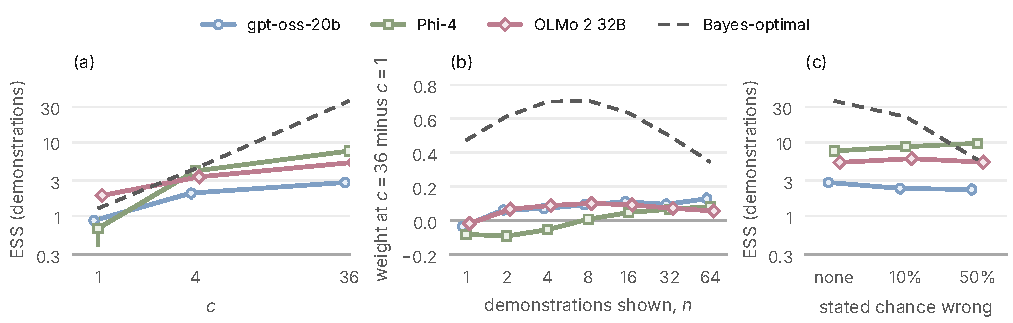
\includegraphics[width=\linewidth]{../../results/llm-test/llm_test.pdf}
\caption{\textbf{The ESS rises with stated specificity, but far less than the Bayes-optimal ESS; stated reliability does not move it; and it falls as demonstrations arrive.} ESS of a description for each model against the Bayes-optimal ESS (dotted), $2{,}000$ tasks, $\sigma = 60$. (a) A relevant description with Bayes-optimal ESS $1$, $4$, or $36$. (b) The description with Bayes-optimal ESS $36$ when it is relevant, when it comes with a stated $10\%$ or $50\%$ chance of being wrong, when it is irrelevant, and when it is irrelevant with a stated $50\%$ chance. In (a) and (b) the ESS is the median over $n = 1$, $2$, and $4$ demonstrations shown, with $95\%$ bootstrap intervals; an irrelevant description's value is an upper bound where Table~\ref{tab:llm} marks it so. (c) The ESS of the relevant description with Bayes-optimal ESS $36$ against the demonstrations shown. In (a) and (c) values at or below $0.3$ are drawn at $0.3$.}
\label{fig:llm}
\end{figure*}

\begin{table*}[t]
\centering\small
\setlength{\tabcolsep}{2.4pt}
\caption{\textbf{The models rely on the stated value by a fixed amount, so a loose description has about its Bayes-optimal ESS and a specific one a small fraction of it.} Left: ESS of a description for each model against its Bayes-optimal ESS, the median over $n = 1$, $2$, and $4$ demonstrations shown ($\sigma = 60$, $2{,}000$ tasks; brackets, $95\%$ bootstrap intervals; negative: the description costs that many demonstrations; $\le$: one demonstration alone beats the description, so the ESS is at most the value shown), for a relevant description with Bayes-optimal ESS $1$, $4$, or $36$, an irrelevant one that would have ESS $36$, and the description with ESS $36$ with a stated $10\%$ or $50\%$ chance of being wrong. Right: the weight on the stated value with one demonstration shown, for the three relevant descriptions; the Bayes-optimal weight is $c/(c+n)$. The Bayes-optimal row knows only what the prompt says, takes a description as relevant unless a reliability is stated, and then hedges with that $p$.}
\label{tab:llm}
\vspace{3pt}
\begin{tabular}{lcccccccccc}
\toprule
& \multicolumn{6}{c}{ESS, median over $n = 1$, $2$, $4$} & & \multicolumn{3}{c}{weight, $n = 1$} \\
\cmidrule(lr){2-7} \cmidrule(lr){9-11}
& \multicolumn{3}{c}{relevant} & \multicolumn{3}{c}{$c = 36$} & & \multicolumn{3}{c}{relevant} \\
\cmidrule(lr){2-4} \cmidrule(lr){5-7} \cmidrule(lr){9-11}
Model & $c = 1$ & $c = 4$ & $c = 36$ & irrelevant & stated 10\% & stated 50\% & & $c = 1$ & $c = 4$ & $c = 36$ \\
\midrule
Bayes-optimal & 1.3 & 4.4 & 36 & $\leq$ $-$1.0 & 22 & 5.8 & & 0.50 & 0.80 & 0.97 \\
\midrule
gpt-oss-20b & 0.9 {\scriptsize[0.7, 1.0]} & 2.0 {\scriptsize[1.7, 2.3]} & 2.8 {\scriptsize[2.6, 3.1]} & $\leq$ $-$0.4 & 2.4 {\scriptsize[1.9, 2.6]} & 2.3 {\scriptsize[1.9, 2.7]} & & 0.53 & 0.48 & 0.49 \\
Phi-4 & 0.7 {\scriptsize[0.4, 0.9]} & 4.1 {\scriptsize[3.5, 4.6]} & 7.6 {\scriptsize[6.5, 8.6]} & $\leq$ $-$1.0 & 8.7 {\scriptsize[7.8, 9.8]} & 9.7 {\scriptsize[8.7, 11]} & & 0.82 & 0.76 & 0.74 \\
OLMo 2 32B & 1.9 {\scriptsize[1.7, 2.1]} & 3.4 {\scriptsize[3.2, 3.9]} & 5.3 {\scriptsize[4.5, 6.3]} & $\leq$ $-$0.6 & 6.0 {\scriptsize[5.6, 7.1]} & 5.4 {\scriptsize[5.0, 6.0]} & & 0.72 & 0.70 & 0.70 \\
gpt-oss-20b (written) & 0.2 {\scriptsize[0.1, 0.4]} & 2.0 {\scriptsize[1.9, 2.6]} & 3.7 {\scriptsize[3.0, 4.4]} & $\leq$ $-$1.0 & 2.4 {\scriptsize[2.1, 2.6]} & 2.3 {\scriptsize[2.1, 2.6]} & & 0.64 & 0.52 & 0.52 \\
Qwen3.5 9B (written) & 0.2 {\scriptsize[$-$0.1, 0.4]} & 2.7 {\scriptsize[2.1, 3.2]} & 4.0 {\scriptsize[3.5, 4.5]} & $\leq$ $-$1.0 & 0.6 {\scriptsize[0.3, 1.0]} & 1.0 {\scriptsize[0.6, 1.5]} & & 0.81 & 0.76 & 0.80 \\
Gemma 4 12B (written) & 0.0 {\scriptsize[$-$0.1, 0.1]} & 0.5 {\scriptsize[0.3, 0.7]} & 1.8 {\scriptsize[1.4, 2.2]} & $\leq$ $-$0.7 & 1.3 {\scriptsize[1.1, 1.6]} & 2.7 {\scriptsize[2.5, 3.1]} & & 0.34 & 0.24 & 0.59 \\
Gemma 4 31B (written) & 0.0 {\scriptsize[0.0, 0.0]} & 0.2 {\scriptsize[0.1, 0.3]} & 1.4 {\scriptsize[1.2, 1.6]} & $\leq$ $-$0.7 & 0.6 {\scriptsize[0.5, 0.7]} & 0.5 {\scriptsize[0.4, 0.6]} & & 0.48 & 0.49 & 0.72 \\
\bottomrule
\end{tabular}

\end{table*}

\paragraph{A loose description has about its Bayes-optimal ESS; a specific one has a small fraction of it.} A description with Bayes-optimal ESS $1$ has an ESS of $0.9$ for gpt-oss-20b, $0.7$ for Phi-4, and $1.9$ for OLMo~2 32B (Table~\ref{tab:llm}). One with Bayes-optimal ESS $4$ has $2.0$, $4.1$, and $3.4$. One with Bayes-optimal ESS $36$ has $2.8$, $7.6$, and $5.3$. The ESS rises with the stated specificity, so the models do respond to specificity, but a description that narrows the mean to within $10$ has an ESS of a few for them and thirty-six for the Bayes-optimal predictor (Figure~\ref{fig:llm}a). The noise-$30$ conditions give the same picture at the same $c$ (Appendix~\ref{app:llm}).

\paragraph{An irrelevant description costs about a demonstration, and a stated chance of being wrong changes nothing.} An irrelevant description that would have ESS $36$ if relevant has an ESS of $-0.5$ for gpt-oss-20b and at most $-1$ and $-0.6$ for Phi-4 and OLMo~2 32B, as for the Bayes-optimal predictor that takes it as relevant. Stating that the description has a $10\%$ or a $50\%$ chance of being wrong leaves its ESS where it was: $2.4$ and $2.3$ for gpt-oss-20b, $8.7$ and $9.7$ for Phi-4, $6.0$ and $5.4$ for OLMo~2 32B, where the Bayes-optimal predictor's hedge gives $22$ and $5.8$ (Figure~\ref{fig:llm}b).

\paragraph{The models rely on the stated value by a fixed amount, then stop.} With no demonstrations shown, the models answer the stated value (weight $0.93$ to $1.00$; Phi-4 and OLMo~2 32B then answer with a number in a fifth and three fifths of replies, and are read from those). With one shown, the weight on the stated value is the same whether the description's Bayes-optimal ESS is $1$, $4$, or $36$: $0.53$, $0.48$, and $0.49$ for gpt-oss-20b, $0.82$, $0.76$, and $0.74$ for Phi-4, and $0.72$, $0.70$, and $0.70$ for OLMo~2 32B, where the Bayes-optimal weight is $0.50$, $0.80$, and $0.97$. The band holds at both noise levels and every $n$ (Table~\ref{tab:llm-full}). Individual replies show the mechanism: a model copies the stated value or copies the average of the demonstrations, and which it copies changes with the demonstrations shown, not with the description. So the ESS of a specific description falls as demonstrations arrive, from $15$ at one demonstration to $4.7$ at four for Phi-4, where the Bayes-optimal ESS stays at $36$ (Figure~\ref{fig:llm}c); the stated specificity raises the ESS only because a more specific description states a value closer to the truth.

\paragraph{Reasoning closes the gap.} Given room to reason before answering, the models move to the Bayes-optimal weight. gpt-oss-20b at low reasoning effort puts a weight of $0.50$, $0.79$, and $0.95$ on the stated value with one demonstration shown, against the Bayes-optimal $0.50$, $0.80$, and $0.97$ ($100$ tasks; Table~\ref{tab:reason}, Appendix~\ref{app:llm}). A frontier model, GPT-5.6-Luna, reached through an agent interface, matches the Bayes-optimal weight to within $0.03$ at every $c$ and $n$, and with its reasoning off shows the fixed weight of the open models (Table~\ref{tab:agent}). The band above is what a model does without computing.

\paragraph{The models learn slowly from demonstrations.} With no description, their error after $64$ demonstrations is $17$ to $20$, against $7.5$ for the Bayes-optimal predictor; this inflates a description's ESS for them, which is small even so.

\section{Conclusion}
We asked how many demonstrations a task description is worth, and answered for the Bayes-optimal predictor in in-context linear regression. A reliable description is worth a number of demonstrations that grows with the task dimension and with the description's specificity. A description that may be irrelevant is worth as much when it is relevant and nothing when it is not, and not knowing which costs at most the entropy of its reliability; a predictor that does not hedge can lose more than the description gives. Networks trained on the task distribution come close to these values for reliable descriptions and take their trust in a description from that distribution. Pretrained language models told a description's specificity and reliability in words use the description, but rely on it by a fixed amount that neither moves, so a description with a Bayes-optimal ESS of thirty-six has an ESS of a few for them; given room to reason, they reach the Bayes-optimal weight. Taken together, the experiments suggest that unless a learner computes, a description's ESS for it is set by its experience of descriptions, not by what the description says about itself. The measure needs only a learner's answers, so the same question can be put to any model.

\paragraph{Limitations.} The analysis assumes a linear-Gaussian task and a description that is equally specific in every direction; a real description can be exact about some aspects of a task and silent about others. The network results rest on one training run per setting, two for one of them, and a network with a mixture output would not meet the single-Gaussian limit. The language-model test covers three small open models and the simplest case of the setting, with one prompt wording. The bound on the price of not knowing whether a description is relevant is specific to log loss.

\section*{Impact Statement}
This paper gives task descriptions a value in demonstrations and tests whether learners honour it, which bears on how instructions and examples are combined in prompts. We see no societal consequences that need specific discussion.

\bibliographystyle{icml2026}
\bibliography{refs}

\clearpage
\onecolumn
\appendix
\section{Proofs}

\subsection{Proof of Theorem \ref{prop:reliable} (Reliable Descriptions)}\label{app:specificity}
We state the theorem in full, with the regret bounds behind (i) and (ii), prove those bounds as two lemmas with their expansions, and then locate the point where the two regret curves cross, which defines the ESS.

\medskip\noindent\textbf{Theorem~\ref{prop:reliable} (Full Statement).} {\itshape Suppose our description is always relevant ($p = 1$), let $\psi$ be the digamma function, and let $c = 1/(r a_0)$, the noise variance divided by the description's prior variance (its ``conjugate-prior ESS'').
\begin{enumerate}
\item[(i)] \emph{Loose descriptions.} For every $n < d$, the baseline regret satisfies $R^{\mathrm{ex}}(n) \ge \tfrac12\big[\log(2a_0) + \psi\big(\tfrac{d-n}{2}\big)\big]$, and the difference tends to $0$ as $a_0 \to \infty$. If the description is vague ($c \le 1$), it is worth roughly $d(1-r)$ demonstrations: as $rd \to \infty$, uniformly in $c \le 1$,
\[
\ess = (d-1)(1-r) + (1-r)\,c + O\!\left(\tfrac{1}{rd}\right).
\]
\item[(ii)] \emph{Specific descriptions.} For every $n \ge d$, the baseline regret satisfies $R^{\mathrm{ex}}(n) \le \Phi(n) := \tfrac12\big[\psi\big(\tfrac{n+1}{2}\big) - \psi\big(\tfrac{n-d+1}{2}\big)\big]$, and the difference tends to $0$ as $a_0 \to \infty$. If $a_0 \ge 1$ and the description is very specific, it is worth roughly $c + d$ demonstrations: as $c/d \to \infty$, uniformly in $a_0 \ge 1$,
\[
\ess = c + d + 1 - \tfrac{1}{a_0} + O\!\left(\tfrac{d}{c}\right).
\]
\item[(iii)] \emph{Hard bound.} No matter the parameters, the description can never be worth more than $c + d + 2$ demonstrations.
\end{enumerate}}
\medskip

\paragraph{Standard facts and notation.}
The noise variance is $1$ throughout. Let $\varepsilon = 1/a_0$ be the precision (inverse variance) of our base prior. When a new query input $x$ arrives, its squared length $A = \|x\|^2$ follows a chi-squared distribution with $d$ degrees of freedom, $A \sim \chi^2_d$. If we have seen $n$ demonstrations, stored as the rows of a matrix $X_n \in \R^{n \times d}$, and no description, our posterior covariance is $\Sigma = (\varepsilon I + X_n^\top X_n)^{-1}$. We often meet the expected log of a predictive variance of the form $1 + At$, which we write $g(t) = \E \log(1 + At)$. This function is increasing and concave, with
\begin{equation}\label{eq:g-derivs}
d\,(1 - (d+2)t) \le g'(t) = \E \frac{A}{1 + At} \le d,
\qquad
-(d^2 + 2d) \le g''(t) \le 0 .
\end{equation}
We use three standard facts about chi-squared and Wishart variables. (S1) $\E \log \chi^2_k = \psi(k/2) + \log 2$, $\E[(\chi^2_k)^{-j}] = \prod_{i=1}^{j} (k - 2i)^{-1}$ for $k > 2j$, and $\psi(z) = \log z - 1/(2z) + O(z^{-2})$. (S2) For $W \sim \mathcal{W}_j(\nu, I)$ with $\nu \ge j$ and $z \sim \mathcal{N}(0, I)$ independent of $W$, $z^\top W^{-1} z$ is distributed as $\chi^2_j / \chi^2_{\nu-j+1}$ with independent numerator and denominator \citep[Theorem~3.2.12]{muirhead1982}, and $\E \operatorname{tr} W^{-2} = j(\nu-1)/((\nu-j)(\nu-j-1)(\nu-j-3))$ for $\nu - j \ge 4$ \citep{vonrosen1988}. (S3) $v - v^2/2 \le \log(1 + v) \le v$ for $v \ge 0$.

\paragraph{Baseline and description regret.}
Our expected regret is tied to how uncertain we are about the query's label. The posterior predictive is the true conditional law of $y$, a Gaussian with variance $1 + x^\top \Sigma x$, so its expected log loss is its entropy, and the regret is half the expected log of the predictive variance. With only the $n$ demonstrations, the baseline regret is $R^{\mathrm{ex}}(n) = \tfrac12 \E \log(1 + x^\top \Sigma x)$. Because each new demonstration adds information, this regret strictly decreases as $n$ grows: by the Sherman--Morrison formula, each new demonstration lowers $x^\top \Sigma x$ almost surely. If we instead have a reliable description and no demonstrations, our covariance is simply $r a_0 I = I/c$; in this subsection we write $R^{\mathrm{desc}}$ for its regret $R^{\mathrm{desc}}_{p=1}(0)$, so by (S1) and (S3) with $v = c/A$,
\begin{equation}\label{eq:rdesc}
2R^{\mathrm{desc}} = g(1/c) = \log(2 r a_0) + \psi(d/2) + \delta^{\mathrm{desc}},
\qquad
\delta^{\mathrm{desc}} = \E \log(1 + c/A) = \frac{c}{d-2} + O\!\left(\frac{c^2}{d^2}\right) \quad (d \ge 5).
\end{equation}
The correction $\delta^{\mathrm{desc}}$ is small when the description is loose ($c$ small) and grows when it is specific.

\paragraph{Locating the ESS.}
To find the ESS, we locate the point where the baseline regret drops to the description regret. Let $h(n) = 2R^{\mathrm{ex}}(n) - 2R^{\mathrm{desc}}$ on integers $n \ge 0$, with linear interpolant $\bar h$. Then $h(0) = g(a_0) - g(r a_0) > 0$, $h$ is strictly decreasing, and $h(n) \to -2R^{\mathrm{desc}} < 0$, since $R^{\mathrm{ex}}(n) \le \Phi(n) \to 0$ by Lemma~\ref{lem:many}; so the ESS is the unique root of $\bar h$. In each regime we show that near the crossing the gap falls at a steady rate $\alpha$: for some $n_0 \ge 0$, $\alpha > 0$, and $\theta \to 0$ along the stated limit,
\begin{equation}\label{eq:root}
h(n) = \alpha\,(n_0 - n) + O(\alpha\theta)
\qquad \text{uniformly over integers $n \ge 0$ with $|n - n_0| \le 3$.}
\end{equation}
Being a convex combination of two such values, $\bar h(t)$ obeys the same expansion at real $t \ge 0$ with $|t - n_0| \le 2$; so for small $\theta$ the root lies within $2$ of $n_0$, and $0 = \bar h(\ess) = \alpha(n_0 - \ess) + O(\alpha\theta)$ gives $\ess = n_0 + O(\theta)$. The approximate root $n_0$ is the value the theorem states.

\begin{lemma}[Baseline Regret with Fewer than $d$ Demonstrations]\label{lem:few}
Suppose we have $n < d$ demonstrations, leaving $k = d - n$ directions completely unseen. Our baseline regret is driven by our prior uncertainty in those unseen directions:
\[
2R^{\mathrm{ex}}(n) = \log(2a_0) + \psi(k/2) + \delta^{\mathrm{ex}},
\]
where the residual $\delta^{\mathrm{ex}} \ge 0$ tends to $0$ as the prior variance $a_0 \to \infty$. For $k \ge 5$ it is proportional to the base prior's precision $\varepsilon = 1/a_0$:
\[
\delta^{\mathrm{ex}} = \frac{\varepsilon (d-1)}{(k-1)(k-2)} + O\!\left(\frac{\varepsilon^2 d^2}{k^4}\right).
\]
\end{lemma}

\begin{proof}
With fewer demonstrations than dimensions, the demonstration inputs span only an $n$-dimensional subspace. In the remaining $k = d - n$ directions the data tell us nothing, so our uncertainty there is the full prior variance $a_0$; in the seen directions the demonstrations have narrowed it. The query's predictive variance therefore splits into an unseen part and a seen part.

Formally, write $X_n^\top X_n = \sum_{i \le n} \lambda_i u_i u_i^\top$ with $\lambda_i > 0$ almost surely, and let $Q$ be the squared length of the projection of $x$ onto the $k$ unseen directions, orthogonal to the $u_i$. Then $\Sigma$ has eigenvalue $a_0$ on those directions and $1/(\varepsilon + \lambda_i)$ on $u_i$, so
\[
1 + x^\top \Sigma x = a_0 Q + T, \qquad T = 1 + V, \quad V = \sum_{i \le n} \frac{z_i^2}{\varepsilon + \lambda_i}, \quad z_i = u_i^\top x,
\]
where, given $X_n$, the $z_i$ are independent standard normals, independent of $Q \sim \chi^2_k$. Factoring out the unseen part $a_0 Q$ and using (S1),
\[
2R^{\mathrm{ex}}(n) = \log(2a_0) + \psi(k/2) + \delta^{\mathrm{ex}}, \qquad \delta^{\mathrm{ex}} = \E \log\!\left(1 + \frac{\varepsilon T}{Q}\right) \ge 0 .
\]
As $a_0 \to \infty$, $\varepsilon T$ decreases to $0$ pathwise, so $\delta^{\mathrm{ex}} \to 0$ by dominated convergence (the integrand at $a_0 = 1$ is integrable).

For the expansion, let $F = \sum_i z_i^2 / \lambda_i$. In the eigenbasis of $W = X_n X_n^\top \sim \mathcal{W}_n(d, I)$, which has the same eigenvalues, $F = z^\top W^{-1} z$ and $\sum_i z_i^2/\lambda_i^2 = z^\top W^{-2} z$ with $z \sim \mathcal{N}(0, I)$ independent of $W$. By (S2), $F \sim \chi^2_n / \chi^2_{k+1}$, so $\E F = n/(k-1)$ and $\E (1+F)^2 = O(d^2/k^2)$, and $\E \sum_i z_i^2/\lambda_i^2 = n(d-1)/(k(k-1)(k-3))$. Since $1/\lambda - \varepsilon/\lambda^2 \le 1/(\varepsilon + \lambda) \le 1/\lambda$, we have $F - \varepsilon \sum_i z_i^2/\lambda_i^2 \le V \le F$. Now (S3) with $v = \varepsilon T / Q$, the independence of $Q$ from $T$, and (S1) give
\[
\frac{\varepsilon\,(1 + \E V)}{k-2} - \frac{\varepsilon^2\, \E T^2}{2(k-2)(k-4)} \le \delta^{\mathrm{ex}} \le \frac{\varepsilon\,(1 + \E F)}{k-2} = \frac{\varepsilon (d-1)}{(k-1)(k-2)} ,
\]
and the two sides differ by at most $\varepsilon^2 \E \sum_i z_i^2/\lambda_i^2 /(k-2) + \varepsilon^2 \E T^2 / (2(k-2)(k-4)) = O(\varepsilon^2 d^2 / k^4)$, as $\E T^2 \le \E (1 + F)^2$.
\end{proof}

\begin{lemma}[Baseline Regret with at Least $d$ Demonstrations]\label{lem:many}
Suppose we have $n \ge d$ demonstrations, so the data span all directions. Let $\ell = n - d + 1$ be the excess degrees of freedom. Then $2\Phi(n) = \E \log(1 + A/Q)$ with $Q \sim \chi^2_\ell$ independent of $A$, the baseline regret satisfies $R^{\mathrm{ex}}(n) \le \Phi(n)$, and the difference tends to $0$ as the prior variance $a_0 \to \infty$. If moreover $a_0 \ge 1$ and $\ell \ge \max(d, 7)$, the prior's precision $\varepsilon = 1/a_0$ lowers the regret slightly:
\[
2R^{\mathrm{ex}}(n) = 2\Phi(n) - \frac{\varepsilon d}{\ell^2} + O\!\left(\frac{\varepsilon d^2}{\ell^3}\right).
\]
\end{lemma}

\begin{proof}
Once $n \ge d$, the data span the entire space, so we are no longer blind in any direction. Because the input distribution is spherically symmetric, we can rotate coordinates so that the query points along the first axis, $x = \|x\| e_1$; the rows of $X_n$ remain independent $\mathcal{N}(0, I_d)$ and independent of $A$. The predictive variance is then $A$ times the first diagonal entry of $\Sigma$: $x^\top \Sigma x = A\,\Sigma_{11} = A/S$, where $S$ is the Schur complement of the first coordinate in $\Sigma^{-1} = \varepsilon I + X_n^\top X_n$. Let $\xi \in \R^n$ be the first column of $X_n$ and $X_-$ its other $d-1$ columns. By the Woodbury identity,
\[
S = \varepsilon + \xi^\top \big(I + a_0 X_- X_-^\top\big)^{-1} \xi .
\]
So $S$ is roughly the squared length of $\xi$ in the directions the other columns leave free. Given $X_-$, the middle matrix has eigenvalue $1$ on the $\ell = n - d + 1$ directions orthogonal to the columns of $X_-$ and $1/(1 + a_0 \mu_j)$ on the other $d - 1$, where $\mu_j$ are the eigenvalues of $M = X_-^\top X_- \sim \mathcal{W}_{d-1}(n, I)$. Since $\xi \sim \mathcal{N}(0, I)$ is independent of $X_-$, its coordinates in that eigenbasis are independent standard normals, and
\[
S = Q + \Delta, \qquad Q \sim \chi^2_\ell, \qquad
\Delta = \varepsilon + \sum_{j < d} \frac{z_j^2}{1 + a_0 \mu_j} \in \big[\varepsilon,\, \varepsilon(1 + F)\big], \qquad F = \sum_{j < d} \frac{z_j^2}{\mu_j},
\]
with $A$, $Q$, and $(z, M)$ independent. The residual $\Delta$ is small and vanishes as $a_0 \to \infty$, so $S \approx Q$. By (S2), $F \sim \chi^2_{d-1} / \chi^2_{\ell+1}$, so $\E F = (d-1)/(\ell-1)$ and, when $\ell \ge \max(d, 7)$, $\E (1+F)^2 \le 5$.

Since $A + Q \sim \chi^2_{n+1}$ and $A/(A+Q)$ is independent of $A+Q$, (S1) gives $\E \log(1 + A/Q) = \psi\big(\tfrac{n+1}{2}\big) - \psi\big(\tfrac{\ell}{2}\big) = 2\Phi(n)$. As $S \ge Q$, $R^{\mathrm{ex}}(n) \le \Phi(n)$, and the difference tends to $0$ as $a_0 \to \infty$ by monotone convergence, since $\Delta$ decreases to $0$.

For the expansion, $2R^{\mathrm{ex}}(n) = 2\Phi(n) - \E G$ with
\[
G = \log\Big(1 + \frac{A}{Q}\Big) - \log\Big(1 + \frac{A}{S}\Big) = \log(1 + v_1) - \log(1 + v_2), \quad v_1 = \frac{\Delta}{Q} \ge v_2 = \frac{\Delta}{Q + A}, \quad v_1 - v_2 = \frac{\Delta A}{Q(Q+A)} .
\]
By concavity of $\log(1+v)$ and $1/(1+v_1) \ge 1 - v_1$, $(v_1 - v_2)(1 - \Delta/Q) \le G \le v_1 - v_2$. Here $\Delta$ is independent of $(A, Q)$; $\E \frac{A}{Q(Q+A)} = \E\frac1Q - \E\frac{1}{Q+A} = \frac{d}{(\ell-2)(\ell+d-2)}$ by (S1), as $Q + A \sim \chi^2_{\ell+d}$; $\frac{A}{Q^2(Q+A)} \le \frac{A}{Q^3}$; and $\varepsilon \le \E\Delta \le \varepsilon(1 + \E F) = \varepsilon\frac{\ell+d-2}{\ell-1}$, $\E \Delta^2 \le 5\varepsilon^2$. Hence
\[
\frac{\varepsilon d}{(\ell-2)(\ell+d-2)} - \frac{5\,\varepsilon^2 d}{(\ell-2)(\ell-4)(\ell-6)} \le \E G \le \frac{\varepsilon d}{(\ell-1)(\ell-2)} ,
\]
and both sides are $\varepsilon d / \ell^2 + O(\varepsilon d^2 / \ell^3)$, using $\varepsilon \le 1$.
\end{proof}

\paragraph{Any prior precision.}
The proof of Lemma~\ref{lem:many} uses $\varepsilon$ only as the precision of the prior, so it applies to any starting precision. For $\kappa > 0$ let $R^{\kappa}(n) = \tfrac12 \E \log\big(1 + x^\top (\kappa I + X_n^\top X_n)^{-1} x\big)$, the regret after $n$ demonstrations under a Gaussian prior of precision $\kappa$ in every direction, so that $R^{\mathrm{ex}} = R^{\varepsilon}$. With $\kappa$ in place of $\varepsilon$ and $1/\kappa$ in place of $a_0$, the same proof gives $\Delta \in [\kappa, \kappa(1+F)]$ and, for $\ell \ge \max(d, 7)$,
\begin{equation}\label{eq:any-tau}
2R^{\kappa}(n) = 2\Phi(n) - \frac{\kappa d}{\ell^2} + O\!\left(\frac{(\kappa + \kappa^2)\, d^2}{\ell^3}\right).
\end{equation}
We use this to compare predictors that start with different prior uncertainties.

\begin{proof}[Proof of Theorem~\ref{prop:reliable}]
\emph{The idea.} In the loose regime the description is worth fewer than $d$ demonstrations, so we compare it with the unseen-directions formula of Lemma~\ref{lem:few}: equating $\log(a_0) + \psi((d - n)/2)$ with $\log(r a_0) + \psi(d/2)$ and using $\psi(z) \approx \log z$ gives $d - n \approx rd$, that is $n \approx d(1-r)$ demonstrations. In the specific regime the description is worth more than $d$ demonstrations, so we compare $\E\log(1 + A/Q)$ from Lemma~\ref{lem:many} with $\E\log(1 + A/c)$: the two match when $\E[1/Q] = 1/(\ell - 2)$ is about $1/c$, that is $n \approx c + d + 1$. The steps below make both comparisons exact up to the stated error.

\emph{(i) Loose descriptions.} The lower bound and the limit follow from Lemma~\ref{lem:few}. For the expansion let $c \le 1$, $n_0 = (d-1)(1-r) + (1-r)c$, and $n \ge 0$ an integer with $|n - n_0| \le 3$; write $k = d - n = rd + u$. Since $n_0 = d - rd - u_0$ with $u_0 = (1-r)(1-c) \in [0, 1]$, we have $|u| \le 4$, so $k \ge 5$ once $rd \ge 9$. By Lemma~\ref{lem:few}, \eqref{eq:rdesc}, $\psi(z) = \log z - 1/(2z) + O(z^{-2})$, and $\varepsilon = rc$, with every $O$ uniform in $c \le 1$ and $|u| \le 4$,
\begin{align*}
h(n) &= \psi(k/2) - \psi(d/2) - \log r + \delta^{\mathrm{ex}} - \delta^{\mathrm{desc}} \\
&= \Big[\log\frac{k}{rd} - \frac1k + \frac1d\Big] + \frac{\varepsilon d}{r^2 d^2}\Big(1 + O\Big(\frac{1}{rd}\Big)\Big) - \frac{c}{d} + O\Big(\frac{1}{(rd)^2}\Big)
 = \frac{u - 1 + r + c - \varepsilon}{rd} + O\Big(\frac{1}{(rd)^2}\Big),
\end{align*}
since $\log(k/(rd)) = u/(rd) + O((rd)^{-2})$, $1/k = 1/(rd) + O((rd)^{-2})$, $\varepsilon d / (r^2 d^2) = c/(rd)$, and $c/d = \varepsilon/(rd)$. So $h(n) = \frac{1}{rd}\big[(n_0 - n) + O(1/(rd))\big]$, which is~\eqref{eq:root} with $\alpha = \theta = 1/(rd)$, and $\ess = (d-1)(1-r) + (1-r)c + O(1/(rd))$.

\emph{(ii) Specific descriptions.} The upper bound and the limit follow from Lemma~\ref{lem:many}. For the expansion let $n_0 = c + d + 1 - \varepsilon$ and $n$ an integer with $|n - n_0| \le 3$, so that $\ell - 2 = c + b$ with $b = n - n_0 - \varepsilon$, $|b| \le 4$; for $c \ge 9d$ every such $n$ has $\ell \ge \max(d, 7)$. By~\eqref{eq:rdesc} and Lemma~\ref{lem:many}, $2\Phi(n) - 2R^{\mathrm{desc}} = \E\big[g(1/Q) - g(1/c)\big]$, and a second-order Taylor expansion of $g$ about $1/c$ with~\eqref{eq:g-derivs}, $\E[1/Q] - 1/c = -b/(c(c+b))$, and $\E(1/Q - 1/c)^2 = \operatorname{Var}(1/Q) + b^2/(c(c+b))^2 = O(c^{-3})$ gives
\[
2\Phi(n) - 2R^{\mathrm{desc}} = -\frac{b}{c(c+b)}\,d\,\Big(1 + O\Big(\frac dc\Big)\Big) + O\Big(\frac{d^2}{c^3}\Big) = -\frac{db}{c^2} + O\Big(\frac{d^2}{c^3}\Big).
\]
With Lemma~\ref{lem:many}, $\varepsilon \le 1$, and $\varepsilon d/\ell^2 = \varepsilon d/c^2 + O(d/c^3)$,
\[
h(n) = -\frac{d}{c^2}\Big[b + \varepsilon + O\Big(\frac{d}{c}\Big)\Big] = \frac{d}{c^2}\Big[(n_0 - n) + O\Big(\frac{d}{c}\Big)\Big],
\]
which is~\eqref{eq:root} with $\alpha = d/c^2$ and $\theta = d/c$, uniformly in $a_0 \ge 1$, so $\ess = c + d + 1 - 1/a_0 + O(d/c)$.

\emph{(iii) The hard bound.} Conditionally on $A$, $\log(1 + Av)$ is concave in $v$, so Jensen's inequality with $\E[1/Q] = 1/(\ell-2)$ gives $2\Phi(n) \le g(1/(\ell-2))$ for $\ell \ge 3$. If $\ell - 2 \ge c$, that is $n \ge c + d + 1$, then $g(1/(\ell-2)) \le g(1/c) = 2R^{\mathrm{desc}}$, so $R^{\mathrm{ex}}(n) \le \Phi(n) \le R^{\mathrm{desc}}$ by Lemma~\ref{lem:many}. The least such integer is $\lceil c + d + 1 \rceil < c + d + 2$, and $R^{\mathrm{ex}}$ is decreasing, so $\ess \le c + d + 2$.
\end{proof}

\subsection{Proof of Proposition \ref{prop:unreliable} (Descriptions That May Be Irrelevant)}\label{app:reliability}
Let $D_n = (x_{1:n}, y_{1:n}, m, x)$ be the prompt with the query input, and let $\pi_n = P(Z = 1 \mid D_n)$ be our current belief that the description is relevant. Write $\pi_n(Z)$ for the belief in the true case: $\pi_n$ if $Z = 1$ and $1 - \pi_n$ otherwise.

\paragraph{Step 1: we must hedge.}
Because we don't know $Z$, our predictive distribution for the new label must hedge: it is a mixture $f(y) = \pi_n f_1(y) + (1 - \pi_n) f_0(y)$, where, given $D_n$, $f_1$ is the Bayes-optimal predictive for a reliable description and $f_0$ the Bayes-optimal predictive from the demonstrations alone; $f_0$ ignores $m$ because an irrelevant description is independent of $w$ and carries no information about $y$. At the start, $\pi_0 = p$: seeing $m$ says nothing about $Z$, because $m$ has the same distribution $\mathcal{N}(0, (1-r) a_0 I)$ in both cases, and $x$ is independent of $Z$.

\paragraph{Step 2: the price of not being told.}
Imagine a ``cheating'' predictor that is secretly told $Z$. It predicts with $f_1$ when $Z=1$, with regret $R^{\mathrm{desc}}_{p=1}(n)$, and with $f_0$ when $Z=0$, with regret $R^{\mathrm{ex}}(n)$, so its expected regret is the weighted average
\[
\text{Cheating Regret} = p\, R^{\mathrm{desc}}_{p=1}(n) + (1-p)\, R^{\mathrm{ex}}(n).
\]
Our honest predictor doesn't know $Z$, so it must use the mixture. Given $(D_n, Z)$ the true density of $y$ is $f_Z$, so the extra regret we suffer is
\[
\E\big[\log f_Z(y) - \log f(y)\big] = \E\big[\mathrm{KL}(f_Z \,\|\, f)\big] = I(Z;\, y \mid D_n) = I_n \ge 0,
\]
the conditional mutual information, because $f$ is the law of $y$ given $D_n$ and $f_Z$ its law given $D_n$ and $Z$. Our total regret is the cheating regret plus $I_n$, which is~\eqref{eq:decomp}.

\paragraph{Step 3: the penalties add up to at most $H(p)$.}
Mutual information is the reduction in uncertainty: $I_n = H(Z \mid D_n) - H(Z \mid D_n, y)$. The query input is independent of $Z$ and of everything else in the prompt, so $H(Z \mid D_n) = H(Z \mid x_{1:n}, y_{1:n}, m)$, and the query with its label is simply one more demonstration, so $H(Z \mid D_n, y) = H(Z \mid D_{n+1})$. Hence $I_n = H(Z \mid D_n) - H(Z \mid D_{n+1})$, the drop in our uncertainty about the description's relevance from step $n$ to step $n+1$. These drops are nonnegative and the sum telescopes; since entropy can never fall below zero, $\sum_{n < N} I_n = H(Z \mid D_0) - H(Z \mid D_N) \le H(Z \mid D_0) = H(p)$, using $\pi_0 = p$ from Step 1.

\paragraph{Step 4: case by case.}
Let the label of each query join the demonstrations, so that $D_{n+1}$ extends $D_n$. By Bayes' rule, $f_Z(y)/f(y) = \pi_{n+1}(Z)/\pi_n(Z)$: the extra log loss on a label is the log of the factor by which that label raises our belief in the true case. Summed over the first $N$ labels, the extra log loss telescopes to $\log \pi_N(Z) - \log \pi_0(Z) \le -\log \pi_0(Z)$. So over the whole prompt we pay at most $\log(1/p)$ more than the cheating predictor when the description is relevant, and at most $\log(1/(1-p))$ more when it is irrelevant.

This completes the proof of Proposition~\ref{prop:unreliable}.

\begin{proof}[Proof of Corollary~\ref{cor:ess}]
\emph{(i) Cap with no demonstrations.} Before seeing any data, \eqref{eq:decomp} with $I_0 \ge 0$ gives $R^{\mathrm{desc}}(0) \ge p\,R^{\mathrm{desc}}_{p=1}(0) + (1-p)\,R^{\mathrm{ex}}(0) \ge (1-p)\,R^{\mathrm{ex}}(0)$ for every $r$, because $R^{\mathrm{desc}}_{p=1}(0) = \tfrac12 \E \log(1 + r a_0 \|x\|^2)$ is nonnegative. However specific the description, the irrelevant case leaves this floor: with probability $1-p$ we suffer the full baseline regret. The baseline regret $R^{\mathrm{ex}}(n)$ strictly decreases and tends to $0$ (Lemma~\ref{lem:many}, as $\Phi(n) \to 0$), so it reaches the floor at a finite number of demonstrations $n^*_p$, defined by $R^{\mathrm{ex}}(n^*_p) = (1-p)\,R^{\mathrm{ex}}(0)$ on the interpolated curve; and since $R^{\mathrm{desc}}(0)$ is at or above the floor, the ESS cannot exceed $n^*_p$, whatever $r$.

\emph{(ii) Discount with many demonstrations.} The idea: with many demonstrations, each further demonstration lowers the baseline regret by about $d/(2n^2)$, and a reliable description lowers it by about $(c - \varepsilon)\,d/(2n^2)$, so it saves about $c - \varepsilon$ demonstrations; a description that is relevant only with probability $p$ saves about $p$ times as much, and the penalty $I_n$ can only lower its value further. To make this exact, fix $d$, $a_0$, and $r$; every $O$ below is as $n \to \infty$ with these fixed. A reliable description leaves the prior $\mathcal{N}(m, r a_0 I)$, of precision $c$ in every direction, and the regret does not depend on $m$, so $R^{\mathrm{desc}}_{p=1} = R^{c}$ in the notation of~\eqref{eq:any-tau}, while $R^{\mathrm{ex}} = R^{\varepsilon}$. Since $1/\ell^2 = 1/n^2 + O(n^{-3})$, \eqref{eq:any-tau} gives
\[
R^{\mathrm{ex}}(n) - R^{\mathrm{desc}}_{p=1}(n) = \frac{(c - \varepsilon)\,d}{2n^2} + O(n^{-3}).
\]
By the standard expansion $\psi(z) = \log z - 1/(2z) - 1/(12z^2) + O(z^{-4})$, $\psi(z + \tfrac12) - \psi(z) = 1/(2z) + 1/(8z^2) + O(z^{-3})$, so $2\Phi(n) - 2\Phi(n+1) = d/(\ell(n+1)) + O(n^{-3})$, and with~\eqref{eq:any-tau} again,
\[
R^{\mathrm{ex}}(n) - R^{\mathrm{ex}}(n+1) = \frac{d}{2n^2} + O(n^{-3}).
\]
Let $L(n) = p\,R^{\mathrm{desc}}_{p=1}(n) + (1-p)\,R^{\mathrm{ex}}(n) = R^{\mathrm{ex}}(n) - p\,\big(R^{\mathrm{ex}}(n) - R^{\mathrm{desc}}_{p=1}(n)\big)$ be the cheating regret, and let $n + s_n$ be the point at which the interpolated $R^{\mathrm{ex}}$ equals $L(n)$. Over any bounded number of steps past $n$ the interpolated $R^{\mathrm{ex}}$ falls by $\tfrac{d}{2n^2}(1 + O(1/n))$ per step, and it must fall by $p\,(c - \varepsilon)\,\tfrac{d}{2n^2}(1 + O(1/n))$ in total, which for large $n$ takes fewer than $\lceil c \rceil + 1$ steps; so $s_n = p\,(c - \varepsilon) + O(1/n)$. If $p = 1$, then $R^{\mathrm{desc}} = L$ and $\ess_n = s_n \to c - \varepsilon$. If $p < 1$, then $R^{\mathrm{desc}}(n) = L(n) + I_n \ge L(n)$ and $R^{\mathrm{ex}}$ is decreasing, so $\ess_n \le s_n$ and $\limsup_n \ess_n \le p\,(c - \varepsilon)$.
\end{proof}

\subsection{The Fully Trusting Predictor}\label{app:trust}
We derive~\eqref{eq:trust}. A ``fully trusting'' predictor always assumes the description is relevant: with no demonstrations, it predicts with variance $v_1 = 1 + r a_0 \|x\|^2$ around the described mean $m^\top x$. Its expected regret depends on whether that assumption is right.
\begin{itemize}
    \item If the description \emph{is} relevant, the predictor's assumptions are correct: its predictive is the true conditional law of $y$, and its regret is the optimal $\tfrac12 \E \log v_1 = R^{\mathrm{desc}}_{p=1}(0)$.
    \item If the description is \emph{irrelevant}, the predictor centers its guess on an unrelated mean. Since $w$ is independent of $m$, given $x$ the error $y - m^\top x$ has mean zero and variance $1 + a_0\|x\|^2 + (1-r)a_0\|x\|^2 = v_1 + 2(1-r)a_0\|x\|^2$: the noise, the variance of $w$, and the variance of $m$. The expected log loss of its Gaussian guess given $x$ is then $\tfrac12 \log(2\pi v_1) + \tfrac12 + (1-r)a_0\|x\|^2/v_1$, against $\tfrac12 \log(2\pi) + \tfrac12$ for the oracle, so its regret given $x$ is $\tfrac12 \log v_1 + (1-r)a_0\|x\|^2/v_1$. Because it guesses with a narrow variance $v_1$ while its error is much larger, it pays the extra $(1-r)a_0\|x\|^2/v_1$.
\end{itemize}
Averaging these two cases with probabilities $p$ and $1-p$ gives~\eqref{eq:trust}. As the description becomes extremely specific ($r \to 0$), the integrand of the penalty increases to $a_0\|x\|^2$, so by monotone convergence the penalty increases to $(1-p)\,a_0 d$: the predictor is confident in an answer that is wrong a fraction $1-p$ of the time.

\section{The Meta-Trained Networks in Full}\label{app:networks}
\paragraph{Training details.} Each demonstration token holds an input beside its label, and two indicator coordinates mark the token type; there is no positional encoding. The Transformer has $12$ layers, $8$ heads, and width $256$, trained with Adam at a learning rate of $10^{-4}$ on fresh prompts at every step, $40{,}000$ steps at batch $1024$ without a curriculum. The number of demonstrations in a training prompt is uniform on $0$ to $20$. The reference predictors are computed once on $200{,}000$ prompts. The full-trust comparison of \S\ref{sec:networks} and the single-Gaussian predictive are described in Table~\ref{tab:networks}'s caption. A network trained at $r = 0.05$, $p = 0.9$ and continued to $80{,}000$ steps kept the shortfall below the Bayes-optimal ESS ($3.9$ against $5.0$). The numerical results of \S\ref{sec:specificity} and \S\ref{sec:reliability} are at one setting, $d = 16$ and $a_0 = 10$; the full-trust formula~\eqref{eq:trust} is for a prompt with no demonstrations, and Corollary~\ref{cor:ess}(ii) is a limit: with few demonstrations in hand, the ESS of a description that may be irrelevant need not be below $p$ times that of a reliable one.
\begin{table}[t]
\centering\small
\caption{Networks against the reference predictors ($d=5$, $a_0=10$; 20{,}000 evaluation prompts per network, with the standard error of its ESS; the last three rows are the second seed). ``Trained'' and ``calibrated'' are the Bayes-optimal predictors with the training and the test reliability, computed once on 200{,}000 prompts (standard errors below $0.12$) and shown once where they coincide; ``single Gaussian'' is the best predictive that a mean and a variance can express, where the Bayes-optimal predictive is a mixture. ``Trust'' is the network's implied trust with the description alone, on a grid of step $0.05$ plus $0.99$ and $0.999$. The last two columns are the mean regret gap, network minus the trained predictor, over $n = 0, \dots, 20$, with and without a description.}
\label{tab:networks}
\vspace{3pt}
\begin{tabular}{rrrrrrrr}
\toprule
& & & \multicolumn{3}{c}{ESS} & \multicolumn{2}{c}{Regret gap (nats)} \\
\cmidrule(lr){4-6}\cmidrule(lr){7-8}
$r$ & $p_{\mathrm{train}}$ & $p_{\mathrm{test}}$ & Network & Trained & Calibrated & Description & None \\
\midrule
0.01 & 1 & 1 & 14.74 & 15.35 & --- & 0.026 & 0.030 \\
0.1 & 1 & 1 & 5.24 & 5.28 & --- & 0.017 & 0.016 \\
0.01 & 0.9 & 0.9 & 4.30 & 6.82 & --- & 0.073 & 0.022 \\
0.1 & 0.9 & 0.9 & 3.57 & 4.22 & --- & 0.034 & 0.018 \\
0.01 & 1 & 0.9 & 0.00 & $\le 0$ & 6.92 & -0.186 & 0.030 \\
0.1 & 1 & 0.9 & 2.32 & 2.05 & 4.26 & 0.010 & 0.016 \\
\bottomrule
\end{tabular}

\end{table}

\section{The Language-Model Test in Full}\label{app:llm}
\paragraph{Measurement.} The ESS of \S\ref{sec:llm} is Definition~\ref{def:ess} with squared error: with $n$ demonstrations shown, the no-description error curve is taken from $n = 1$ on (at $n = 0$ the models rarely answer with a number), made non-increasing, and interpolated in $\log n$; when one demonstration alone beats the description we report the bound $\ess_n \le 1 - n$. The Bayes-optimal yardstick is the predictor that knows only what the prompt says: the noise, the description taken as relevant (with the stated probability where one is given), and otherwise a mean uniform over $100$ to $999$, so that without a description its prediction is the mean of the demonstrations shown. A relevant description's exact Bayes-optimal ESS is then $c$, that is $1$, $4$, and $36$; computed the same way as the models' it reads $1.3$, $4.4$, and $36$, the interpolation biasing it upward by under half a demonstration, and the tables report the computed value for it and the models alike. Where a model answers with a number in fewer than three quarters of the replies of a condition, the prediction is read from a minority of its replies and the tables set the cell in italics. MiniCPM5~2B \citep{minicpm5} and OLMo~2 7B and 13B Instruct begin fewer than three quarters of their replies with a number overall, mostly explaining instead (``To predict\ldots'', ``Given\ldots'') despite the instruction to reply with the number only, and are not reported beyond that. OLMo~2 32B answers with a number in $41\%$ of the no-description prompts with one demonstration shown and $75\%$ with two, so its no-description error at $n = 1$ is read from a minority of its replies. Thinking is disabled where the chat template allows it, and gpt-oss-20b's reply is placed in its final channel.

\paragraph{Prompt variants.} The second sentence of the prompt is ``Its mean is unknown.'' without a description, ``Its mean was drawn from a normal distribution with mean $m$ and standard deviation $\tau$.'' with one, and for an irrelevant description the same with the value of an independently drawn task; a stated reliability adds ``There is a 10\% chance that this statement is wrong, in which case the mean is unknown.'' or the same with 50\%; with no demonstrations the question is ``Predict the first number.'' The noise-$30$ conditions, which realize the same three $c$ with every number in the prompt halved, give ESS values within the intervals of the noise-$60$ ones at the same $c$ and $n$ (Table~\ref{tab:llm-worth}).

Table~\ref{tab:llm-worth} gives the ESS of every description at every number of demonstrations shown, and Table~\ref{tab:llm-full} the weight on the stated value, each against the Bayes-optimal value, with how often each model's reply begins with a number.

\begin{table}[t]
\centering\scriptsize
\setlength{\tabcolsep}{1.2pt}
\caption{ESS of a description, model/Bayes-optimal, for every condition and number of demonstrations shown ($2{,}000$ tasks). ``Number'' is the share of replies that begin with a three-digit number, averaged over $n$; a cell is in italics where that share is below three quarters at that $n$. Rel./irrel.: a relevant or irrelevant description; w.: a stated chance of being wrong. Rel.\ and irrel.: a relevant or an irrelevant description; w.: a stated chance of being wrong. $> 64$: the model's error with the description is below its error with $64$ demonstrations and no description.}
\label{tab:llm-worth}
\vspace{3pt}
\begin{tabular}{llrrrrrrrr}
\toprule
Predictor & Description & number & $n = 1$ & $n = 2$ & $n = 4$ & $n = 8$ & $n = 16$ & $n = 32$ & $n = 64$ \\
\midrule
Bayes-optimal & $\sigma = 60$, $c = 1$, relevant &  & 1.2 & 1.3 & 1.3 & 1.3 & 1.2 & 1.5 & $> 0$ \\
 & $\sigma = 60$, $c = 1$, irrelevant &  & $\leq$ 0.0 & $-$0.5 & $-$0.8 & $-$1.2 & $-$1.7 & $-$1.5 & $-$1.7 \\
 & $\sigma = 60$, $c = 4$, relevant &  & 4.5 & 4.4 & 3.9 & 4.6 & 4.6 & 5.2 & $> 0$ \\
 & $\sigma = 60$, $c = 4$, irrelevant &  & $\leq$ 0.0 & $\leq$ $-$1.0 & $\leq$ $-$3.0 & $-$6.2 & $-$12 & $-$20 & $-$32 \\
 & $\sigma = 60$, $c = 36$, relevant &  & 36 & 36 & 37 & 38 & 39 & $> 32$ & $> 0$ \\
 & $\sigma = 60$, $c = 36$, irrelevant &  & $\leq$ 0.0 & $\leq$ $-$1.0 & $\leq$ $-$3.0 & $\leq$ $-$7.0 & $\leq$ $-$15 & $\leq$ $-$31 & $-$62 \\
 & $\sigma = 30$, $c = 1$, relevant &  & 1.0 & 1.2 & 1.4 & 1.6 & 1.4 & 1.5 & $> 0$ \\
 & $\sigma = 30$, $c = 4$, relevant &  & 4.5 & 4.7 & 5.0 & 5.1 & 4.9 & 5.6 & $> 0$ \\
 & $\sigma = 30$, $c = 36$, relevant &  & 42 & 43 & 43 & 43 & 42 & $> 32$ & $> 0$ \\
 & $\sigma = 60$, $c = 4$, relevant, 10\% wrong &  & 3.8 & 3.9 & 3.6 & 4.4 & 4.5 & 5.1 & $> 0$ \\
 & $\sigma = 60$, $c = 4$, irrelevant, 10\% wrong &  & $\leq$ 0.0 & $-$0.7 & $-$1.2 & $-$1.6 & $-$2.2 & $-$1.9 & $-$2.2 \\
 & $\sigma = 60$, $c = 36$, relevant, 10\% wrong &  & 13 & 22 & 26 & 35 & 38 & $> 32$ & $> 0$ \\
 & $\sigma = 60$, $c = 36$, irrelevant, 10\% wrong &  & $\leq$ 0.0 & $-$0.9 & $-$1.7 & $-$2.8 & $-$5.4 & $-$6.9 & $-$10 \\
 & $\sigma = 60$, $c = 4$, relevant, 50\% wrong &  & 1.9 & 2.2 & 2.9 & 3.7 & 4.1 & 4.5 & $> 0$ \\
 & $\sigma = 60$, $c = 4$, irrelevant, 50\% wrong &  & $\leq$ 0.0 & $-$0.2 & $-$0.4 & $-$0.5 & $-$0.8 & $-$0.6 & $-$0.7 \\
 & $\sigma = 60$, $c = 36$, relevant, 50\% wrong &  & 3.1 & 5.8 & 12 & 21 & 31 & $> 32$ & $> 0$ \\
 & $\sigma = 60$, $c = 36$, irrelevant, 50\% wrong &  & $\leq$ 0.0 & $-$0.3 & $-$0.7 & $-$1.2 & $-$2.4 & $-$2.8 & $-$4.5 \\
\midrule
gpt-oss-20b & $\sigma = 60$, $c = 1$, relevant & 0.98 & 1.0 & 0.9 & $-$0.1 & $-$1.5 & $-$9.2 & $-$25 & $-$57 \\
 & $\sigma = 60$, $c = 1$, irrelevant & 0.98 & $\leq$ 0.0 & $-$0.3 & $-$1.5 & $-$3.6 & $-$10 & $-$25 & $-$59 \\
 & $\sigma = 60$, $c = 4$, relevant & 0.98 & 2.3 & 1.7 & 2.0 & 2.9 & $-$7.5 & $-$24 & $-$48 \\
 & $\sigma = 60$, $c = 4$, irrelevant & 0.97 & $\leq$ 0.0 & $-$0.3 & $-$1.4 & $-$3.7 & $-$11 & $-$26 & $-$59 \\
 & $\sigma = 60$, $c = 36$, relevant & 0.98 & 2.8 & 2.3 & 3.8 & 17 & 3.7 & $-$12 & $-$17 \\
 & $\sigma = 60$, $c = 36$, irrelevant & 0.98 & $\leq$ 0.0 & $-$0.5 & $-$1.5 & $-$3.7 & $-$11 & $-$26 & $-$60 \\
 & $\sigma = 30$, $c = 1$, relevant & 0.99 & 0.8 & 0.4 & $-$0.3 & $-$1.8 & $-$9.9 & $-$26 & $-$59 \\
 & $\sigma = 30$, $c = 4$, relevant & 0.98 & 1.2 & 1.3 & 1.9 & 3.4 & $-$8.1 & $-$24 & $-$44 \\
 & $\sigma = 30$, $c = 36$, relevant & 0.99 & 1.6 & 2.3 & 4.7 & 31 & 3.0 & $-$13 & $> 0$ \\
 & $\sigma = 60$, $c = 4$, relevant, 10\% wrong & 0.96 & 2.2 & 1.8 & 0.0 & $-$0.2 & $-$8.1 & $-$24 & $-$52 \\
 & $\sigma = 60$, $c = 4$, irrelevant, 10\% wrong & 0.96 & $\leq$ 0.0 & $-$0.6 & $-$1.1 & $-$2.2 & $-$9.6 & $-$25 & $-$58 \\
 & $\sigma = 60$, $c = 36$, relevant, 10\% wrong & 0.97 & 2.4 & 2.4 & 0.5 & 2.8 & $-$3.6 & $-$20 & $-$33 \\
 & $\sigma = 60$, $c = 36$, irrelevant, 10\% wrong & 0.96 & $\leq$ 0.0 & $-$0.7 & $-$1.1 & $-$2.3 & $-$9.7 & $-$25 & $-$59 \\
 & $\sigma = 60$, $c = 4$, relevant, 50\% wrong & 0.95 & 2.3 & 1.7 & 0.1 & $-$0.5 & $-$8.3 & $-$24 & $-$53 \\
 & $\sigma = 60$, $c = 4$, irrelevant, 50\% wrong & 0.94 & $\leq$ 0.0 & $-$0.5 & $-$1.1 & $-$2.3 & $-$9.7 & $-$25 & $-$58 \\
 & $\sigma = 60$, $c = 36$, relevant, 50\% wrong & 0.95 & 2.8 & 2.3 & 0.7 & 1.2 & $-$4.5 & $-$21 & $-$37 \\
 & $\sigma = 60$, $c = 36$, irrelevant, 50\% wrong & 0.95 & $\leq$ 0.0 & $-$0.6 & $-$1.1 & $-$2.3 & $-$9.7 & $-$25 & $-$59 \\
\midrule
Phi-4 & $\sigma = 60$, $c = 1$, relevant & 0.87 & 0.8 & 0.7 & $-$0.2 & $-$0.4 & $-$1.0 & $-$2.9 & $-$34 \\
 & $\sigma = 60$, $c = 1$, irrelevant & 0.86 & $\leq$ 0.0 & $\leq$ $-$1.0 & $\leq$ $-$3.0 & $-$4.9 & $-$6.1 & $-$8.7 & $-$40 \\
 & $\sigma = 60$, $c = 4$, relevant & 0.85 & 5.8 & 4.1 & 2.4 & 2.1 & 0.7 & $-$4.4 & $-$33 \\
 & $\sigma = 60$, $c = 4$, irrelevant & 0.84 & $\leq$ 0.0 & $\leq$ $-$1.0 & $\leq$ $-$3.0 & $-$4.7 & $-$6.2 & $-$13 & $-$42 \\
 & $\sigma = 60$, $c = 36$, relevant & 0.86 & 15 & 7.6 & 4.7 & 5.6 & 8.6 & $> 32$ & $> 0$ \\
 & $\sigma = 60$, $c = 36$, irrelevant & 0.84 & $\leq$ 0.0 & $\leq$ $-$1.0 & $\leq$ $-$3.0 & $-$4.5 & $-$6.4 & $-$12 & $-$42 \\
 & $\sigma = 30$, $c = 1$, relevant & 0.87 & 1.1 & 0.8 & $-$0.3 & $-$0.3 & $-$1.0 & $-$1.8 & $-$15 \\
 & $\sigma = 30$, $c = 4$, relevant & 0.86 & 4.8 & 3.5 & 2.0 & 1.6 & 0.6 & $-$1.9 & $-$2.2 \\
 & $\sigma = 30$, $c = 36$, relevant & 0.88 & 9.7 & 6.0 & 3.8 & 4.4 & 8.4 & 17 & $> 0$ \\
 & $\sigma = 60$, $c = 4$, relevant, 10\% wrong & 0.87 & 6.0 & 5.5 & 5.3 & 8.3 & 16 & $> 32$ & $> 0$ \\
 & $\sigma = 60$, $c = 4$, irrelevant, 10\% wrong & 0.85 & $\leq$ 0.0 & $\leq$ $-$1.0 & $-$2.1 & $-$1.2 & 2.9 & $-$3.1 & $> 0$ \\
 & $\sigma = 60$, $c = 36$, relevant, 10\% wrong & 0.87 & 10 & 8.7 & 8.2 & 17 & $> 48$ & $> 32$ & $> 0$ \\
 & $\sigma = 60$, $c = 36$, irrelevant, 10\% wrong & 0.86 & $\leq$ 0.0 & $\leq$ $-$1.0 & $-$2.4 & $-$1.7 & 1.3 & $-$4.5 & $> 0$ \\
 & $\sigma = 60$, $c = 4$, relevant, 50\% wrong & 0.87 & 6.0 & 6.4 & 7.7 & 17 & $> 48$ & $> 32$ & $> 0$ \\
 & $\sigma = 60$, $c = 4$, irrelevant, 50\% wrong & 0.85 & $\leq$ 0.0 & $\leq$ $-$1.0 & $-$1.3 & 1.5 & 16 & $> 32$ & $> 0$ \\
 & $\sigma = 60$, $c = 36$, relevant, 50\% wrong & 0.88 & 9.2 & 9.7 & 11 & $> 56$ & $> 48$ & $> 32$ & $> 0$ \\
 & $\sigma = 60$, $c = 36$, irrelevant, 50\% wrong & 0.86 & $\leq$ 0.0 & $\leq$ $-$1.0 & $-$1.8 & 0.6 & 13 & $> 32$ & $> 0$ \\
\midrule
OLMo 2 32B & $\sigma = 60$, $c = 1$, relevant & 0.90 & 1.9 & 1.8 & 2.0 & 2.3 & 5.8 & $> 32$ & $> 0$ \\
 & $\sigma = 60$, $c = 1$, irrelevant & 0.89 & $\leq$ 0.0 & $-$0.5 & $-$0.2 & $-$0.2 & 1.7 & 25 & $> 0$ \\
 & $\sigma = 60$, $c = 4$, relevant & 0.91 & 5.8 & 3.4 & 3.4 & 4.5 & 9.3 & $> 32$ & $> 0$ \\
 & $\sigma = 60$, $c = 4$, irrelevant & 0.90 & $\leq$ 0.0 & $-$0.7 & $-$0.3 & $-$0.5 & 0.3 & 17 & $> 0$ \\
 & $\sigma = 60$, $c = 36$, relevant & 0.91 & 11 & 4.6 & 5.3 & 6.8 & 15 & $> 32$ & $> 0$ \\
 & $\sigma = 60$, $c = 36$, irrelevant & 0.90 & $\leq$ 0.0 & $\leq$ $-$1.0 & $-$0.6 & $-$0.5 & $-$0.2 & 15 & $> 0$ \\
 & $\sigma = 30$, $c = 1$, relevant & 0.92 & 1.8 & 1.9 & 1.7 & 1.7 & 4.4 & 24 & $> 0$ \\
 & $\sigma = 30$, $c = 4$, relevant & 0.92 & 4.8 & 3.3 & 3.1 & 4.0 & 9.5 & $> 32$ & $> 0$ \\
 & $\sigma = 30$, $c = 36$, relevant & 0.93 & 7.0 & 4.4 & 4.0 & 5.9 & 14 & $> 32$ & $> 0$ \\
 & $\sigma = 60$, $c = 4$, relevant, 10\% wrong & 0.96 & 6.0 & 4.6 & 3.8 & 4.5 & 5.8 & 23 & $> 0$ \\
 & $\sigma = 60$, $c = 4$, irrelevant, 10\% wrong & 0.96 & $\leq$ 0.0 & $-$0.9 & 0.0 & 0.0 & $-$0.4 & 4.1 & $> 0$ \\
 & $\sigma = 60$, $c = 36$, relevant, 10\% wrong & 0.96 & 12 & 5.9 & 6.0 & 6.3 & 8.9 & 31 & $> 0$ \\
 & $\sigma = 60$, $c = 36$, irrelevant, 10\% wrong & 0.96 & $\leq$ 0.0 & $\leq$ $-$1.0 & $-$0.3 & $-$0.1 & $-$0.8 & 0.3 & $> 0$ \\
 & $\sigma = 60$, $c = 4$, relevant, 50\% wrong & 0.93 & 5.3 & 4.2 & 3.5 & 4.0 & 5.4 & 27 & $> 0$ \\
 & $\sigma = 60$, $c = 4$, irrelevant, 50\% wrong & 0.92 & $\leq$ 0.0 & $-$0.5 & 0.1 & 0.1 & 0.0 & 11 & $> 0$ \\
 & $\sigma = 60$, $c = 36$, relevant, 50\% wrong & 0.93 & 7.8 & 5.4 & 4.9 & 5.6 & 7.9 & $> 32$ & $> 0$ \\
 & $\sigma = 60$, $c = 36$, irrelevant, 50\% wrong & 0.92 & $\leq$ 0.0 & $-$0.8 & $-$0.1 & 0.0 & $-$0.3 & 7.8 & $> 0$ \\
\bottomrule
\end{tabular}

\end{table}

\paragraph{Reasoning.} gpt-oss-20b was also run with its reasoning on at low effort, on the first $100$ tasks, with $384$ new tokens and the reply read from its final channel, for seven conditions at $n = 1$ and $4$ (Table~\ref{tab:reason}). It answers with a number less often when it reasons, in a third to a half of replies when a reliability is stated, where the budget runs out before the answer; those cells are set in italics. Where it answers, its weight on the stated value is the Bayes-optimal weight to within $0.02$ for a relevant description at $n = 1$, it discounts an irrelevant one a little ($0.91$ against $0.97$ for the predictor that takes it as relevant), and with a stated $50\%$ chance of being wrong it hedges, to $0.70$ where the Bayes-optimal hedge is $0.57$, which no model does without reasoning.

\begin{table}[h]
\centering\small
\caption{\textbf{With reasoning, gpt-oss-20b puts the Bayes-optimal weight on the stated value.} Low reasoning effort, $100$ tasks, $\sigma = 60$. Number: the fraction of replies that are a number. Weight and error: the model's against the Bayes-optimal predictor's, which hedges with the stated $p$ where one is given. Italics: fewer than three quarters of the replies are a number.}
\label{tab:reason}
\begin{tabular}{lcccccc}
\toprule
& \multicolumn{3}{c}{$n = 1$} & \multicolumn{3}{c}{$n = 4$} \\
\cmidrule(lr){2-4} \cmidrule(lr){5-7}
Description & number & weight & error & number & weight & error \\
\midrule
no description & 1.00 & -- & 60/60 & 1.00 & -- & 30/30 \\
rel. $\tau = 60$ & 1.00 & 0.50/0.50 & 45/45 & 0.80 & 0.13/0.20 & 34/28 \\
rel. $\tau = 30$ & 0.96 & 0.79/0.80 & 28/27 & 0.71 & \textit{0.52/0.50} & \textit{23/22} \\
rel. $\tau = 10$ & 0.93 & 0.95/0.97 & 13/9 & 0.87 & 0.88/0.90 & 10/9 \\
irrel. $\tau = 10$ & 0.94 & 0.91/0.97 & 119/122 & 0.78 & 0.84/0.90 & 113/113 \\
rel. $\tau = 10$, 10\% w. & 0.54 & \textit{0.96/0.86} & \textit{11/14} & 0.43 & \textit{0.74/0.83} & \textit{22/10} \\
rel. $\tau = 10$, 50\% w. & 0.33 & \textit{0.70/0.57} & \textit{28/28} & 0.28 & \textit{0.77/0.64} & \textit{18/14} \\
\bottomrule
\end{tabular}

\end{table}

\paragraph{A frontier model inside an agent harness.} The models above are open ones run locally, so that their first-token distributions can be read. The squared-error ESS needs only answers, so we also put the prompts of three relevant descriptions ($c = 1$, $4$, $36$; $\sigma = 60$) with $n = 1$ and $4$ demonstrations, $100$ tasks each, to GPT-5.6-Luna through the Codex command-line agent on a subscription, once with its reasoning effort set to low (about $135$ reasoning tokens per answer) and once with reasoning off. This measures the model as deployed in that agent: its instructions and tool definitions, about $27{,}000$ tokens, surround the prompt, as a provider's system prompt surrounds it through an API; the model used no tool in any reply, and every one of the $1{,}200$ replies is a bare number. With reasoning, the weight on the stated value is the Bayes-optimal $c/(c+n)$ to within $0.03$ in all six cells, the implied worth $n\,a/b$ is $c$ to within half a demonstration, and the error equals the Bayes-optimal predictor's (Table~\ref{tab:agent}): the prompt contains what is needed to reach the Bayes-optimal ESS, and a model that computes reaches it, whatever surrounds the prompt. With reasoning off, the same model shows the band of \S\ref{sec:llm}: a weight of $0.72$ to $0.88$ at $n = 1$ and $0.40$ to $0.47$ at $n = 4$ whatever the stated specificity, and an implied worth of $2.6$ to $5.8$ demonstrations for descriptions worth $1$ to $36$.

\begin{table}[h]
\centering\small
\caption{\textbf{A frontier model reaches the Bayes-optimal weight when it reasons and shows the fixed weight of the open models when it does not.} GPT-5.6-Luna inside the Codex agent harness, $100$ tasks per cell, relevant descriptions at $\sigma = 60$; weight on the stated value and implied worth $n\,a/b$ from the regression of \S\ref{sec:llm}; bootstrap standard errors of the weights are at most $0.03$ with reasoning and $0.07$ without.}
\label{tab:agent}
\begin{tabular}{lcccccccccccc}
\toprule
& \multicolumn{6}{c}{weight on the stated value} & \multicolumn{6}{c}{implied worth, demonstrations} \\
\cmidrule(lr){2-7} \cmidrule(lr){8-13}
& \multicolumn{3}{c}{$n = 1$} & \multicolumn{3}{c}{$n = 4$} & \multicolumn{3}{c}{$n = 1$} & \multicolumn{3}{c}{$n = 4$} \\
\cmidrule(lr){2-4} \cmidrule(lr){5-7} \cmidrule(lr){8-10} \cmidrule(lr){11-13}
Bayes-optimal ESS $c$ & 1 & 4 & 36 & 1 & 4 & 36 & 1 & 4 & 36 & 1 & 4 & 36 \\
\midrule
Bayes-optimal & 0.50 & 0.80 & 0.97 & 0.20 & 0.50 & 0.90 & 1 & 4 & 36 & 1 & 4 & 36 \\
GPT-5.6-Luna, low reasoning & 0.50 & 0.77 & 0.97 & 0.21 & 0.50 & 0.90 & 1.0 & 3.6 & 36.3 & 1.0 & 4.0 & 36.1 \\
GPT-5.6-Luna, reasoning off & 0.79 & 0.72 & 0.88 & 0.43 & 0.40 & 0.47 & 3.6 & 2.6 & 5.8 & 3.1 & 2.7 & 3.7 \\
\bottomrule
\end{tabular}

\end{table}

\begin{table}[t]
\centering\scriptsize
\setlength{\tabcolsep}{2.5pt}
\caption{Weight on the stated value, model/Bayes-optimal, for every condition and number of demonstrations shown. Italics as in Table~\ref{tab:llm-worth}.}
\label{tab:llm-full}
\vspace{3pt}
\begin{tabular}{llrrrrrrrrr}
\toprule
Predictor & Description & number & $n = 0$ & $n = 1$ & $n = 2$ & $n = 4$ & $n = 8$ & $n = 16$ & $n = 32$ & $n = 64$ \\
\midrule
Bayes-optimal & $\sigma = 60$, $c = 1$, relevant &  & 1.00 & 0.50 & 0.33 & 0.20 & 0.11 & 0.06 & 0.03 & 0.02 \\
 & $\sigma = 60$, $c = 1$, irrelevant &  & 1.00 & 0.50 & 0.33 & 0.20 & 0.11 & 0.06 & 0.03 & 0.02 \\
 & $\sigma = 60$, $c = 4$, relevant &  & 1.00 & 0.80 & 0.67 & 0.50 & 0.33 & 0.20 & 0.11 & 0.06 \\
 & $\sigma = 60$, $c = 4$, irrelevant &  & 1.00 & 0.80 & 0.67 & 0.50 & 0.33 & 0.20 & 0.11 & 0.06 \\
 & $\sigma = 60$, $c = 36$, relevant &  & 1.00 & 0.97 & 0.95 & 0.90 & 0.82 & 0.69 & 0.53 & 0.36 \\
 & $\sigma = 60$, $c = 36$, irrelevant &  & 1.00 & 0.97 & 0.95 & 0.90 & 0.82 & 0.69 & 0.53 & 0.36 \\
 & $\sigma = 30$, $c = 1$, relevant &  & 1.00 & 0.50 & 0.33 & 0.20 & 0.11 & 0.06 & 0.03 & 0.02 \\
 & $\sigma = 30$, $c = 4$, relevant &  & 1.00 & 0.80 & 0.67 & 0.50 & 0.33 & 0.20 & 0.11 & 0.06 \\
 & $\sigma = 30$, $c = 36$, relevant &  & 1.00 & 0.97 & 0.95 & 0.90 & 0.82 & 0.69 & 0.53 & 0.36 \\
 & $\sigma = 60$, $c = 4$, relevant, 10\% wrong &  & 0.90 & 0.71 & 0.59 & 0.45 & 0.30 & 0.19 & 0.10 & 0.05 \\
 & $\sigma = 60$, $c = 4$, irrelevant, 10\% wrong &  & 0.90 & 0.27 & 0.14 & 0.08 & 0.04 & 0.02 & 0.01 & 0.00 \\
 & $\sigma = 60$, $c = 36$, relevant, 10\% wrong &  & 0.90 & 0.84 & 0.84 & 0.82 & 0.77 & 0.65 & 0.51 & 0.34 \\
 & $\sigma = 60$, $c = 36$, irrelevant, 10\% wrong &  & 0.90 & 0.26 & 0.14 & 0.07 & 0.03 & 0.01 & 0.00 & 0.00 \\
 & $\sigma = 60$, $c = 4$, relevant, 50\% wrong &  & 0.50 & 0.46 & 0.39 & 0.32 & 0.22 & 0.14 & 0.08 & 0.04 \\
 & $\sigma = 60$, $c = 4$, irrelevant, 50\% wrong &  & 0.50 & 0.12 & 0.07 & 0.03 & 0.02 & 0.01 & 0.00 & 0.00 \\
 & $\sigma = 60$, $c = 36$, relevant, 50\% wrong &  & 0.50 & 0.55 & 0.58 & 0.60 & 0.59 & 0.53 & 0.42 & 0.29 \\
 & $\sigma = 60$, $c = 36$, irrelevant, 50\% wrong &  & 0.50 & 0.12 & 0.06 & 0.03 & 0.01 & 0.00 & 0.00 & 0.00 \\
\midrule
gpt-oss-20b & $\sigma = 60$, $c = 1$, relevant & 0.98 & 0.94 & 0.53 & 0.29 & 0.23 & 0.16 & 0.12 & 0.12 & 0.23 \\
 & $\sigma = 60$, $c = 1$, irrelevant & 0.98 & 0.93 & 0.59 & 0.25 & 0.18 & 0.09 & 0.05 & 0.04 & 0.10 \\
 & $\sigma = 60$, $c = 4$, relevant & 0.98 & 0.92 & 0.48 & 0.32 & 0.26 & 0.21 & 0.19 & 0.18 & 0.31 \\
 & $\sigma = 60$, $c = 4$, irrelevant & 0.97 & 0.92 & 0.57 & 0.25 & 0.16 & 0.08 & 0.04 & 0.04 & 0.09 \\
 & $\sigma = 60$, $c = 36$, relevant & 0.98 & 0.94 & 0.49 & 0.35 & 0.30 & 0.25 & 0.23 & 0.22 & 0.35 \\
 & $\sigma = 60$, $c = 36$, irrelevant & 0.98 & 0.95 & 0.60 & 0.25 & 0.15 & 0.07 & 0.04 & 0.04 & 0.09 \\
 & $\sigma = 30$, $c = 1$, relevant & 0.99 & 0.98 & 0.43 & 0.23 & 0.17 & 0.12 & 0.09 & 0.11 & 0.21 \\
 & $\sigma = 30$, $c = 4$, relevant & 0.98 & 0.98 & 0.38 & 0.28 & 0.23 & 0.19 & 0.18 & 0.19 & 0.31 \\
 & $\sigma = 30$, $c = 36$, relevant & 0.99 & 0.99 & 0.37 & 0.32 & 0.27 & 0.23 & 0.22 & 0.24 & 0.37 \\
 & $\sigma = 60$, $c = 4$, relevant, 10\% wrong & 0.96 & 0.91 & 0.45 & 0.33 & 0.15 & 0.13 & 0.12 & 0.13 & 0.22 \\
 & $\sigma = 60$, $c = 4$, irrelevant, 10\% wrong & 0.96 & 0.91 & 0.55 & 0.34 & 0.11 & 0.05 & 0.02 & 0.02 & 0.04 \\
 & $\sigma = 60$, $c = 36$, relevant, 10\% wrong & 0.97 & 0.92 & 0.44 & 0.34 & 0.17 & 0.15 & 0.15 & 0.16 & 0.25 \\
 & $\sigma = 60$, $c = 36$, irrelevant, 10\% wrong & 0.96 & 0.92 & 0.53 & 0.34 & 0.10 & 0.04 & 0.02 & 0.02 & 0.04 \\
 & $\sigma = 60$, $c = 4$, relevant, 50\% wrong & 0.95 & 0.79 & 0.46 & 0.32 & 0.16 & 0.12 & 0.12 & 0.12 & 0.20 \\
 & $\sigma = 60$, $c = 4$, irrelevant, 50\% wrong & 0.94 & 0.79 & 0.53 & 0.32 & 0.11 & 0.04 & 0.02 & 0.01 & 0.04 \\
 & $\sigma = 60$, $c = 36$, relevant, 50\% wrong & 0.95 & 0.83 & 0.46 & 0.32 & 0.17 & 0.14 & 0.15 & 0.15 & 0.23 \\
 & $\sigma = 60$, $c = 36$, irrelevant, 50\% wrong & 0.95 & 0.83 & 0.53 & 0.31 & 0.11 & 0.04 & 0.02 & 0.02 & 0.04 \\
\midrule
Phi-4 & $\sigma = 60$, $c = 1$, relevant & 0.87 & \textit{0.97} & 0.82 & 0.62 & 0.43 & 0.28 & 0.18 & 0.13 & 0.12 \\
 & $\sigma = 60$, $c = 1$, irrelevant & 0.86 & \textit{0.97} & 0.83 & 0.64 & 0.42 & 0.22 & 0.11 & 0.06 & 0.05 \\
 & $\sigma = 60$, $c = 4$, relevant & 0.85 & \textit{0.98} & 0.76 & 0.55 & 0.37 & 0.26 & 0.19 & 0.15 & 0.16 \\
 & $\sigma = 60$, $c = 4$, irrelevant & 0.84 & \textit{0.98} & 0.79 & 0.56 & 0.36 & 0.18 & 0.09 & 0.06 & 0.05 \\
 & $\sigma = 60$, $c = 36$, relevant & 0.86 & \textit{0.99} & 0.74 & 0.53 & 0.38 & 0.29 & 0.23 & 0.20 & 0.20 \\
 & $\sigma = 60$, $c = 36$, irrelevant & 0.84 & \textit{0.99} & 0.78 & 0.53 & 0.33 & 0.16 & 0.09 & 0.06 & 0.04 \\
 & $\sigma = 30$, $c = 1$, relevant & 0.87 & \textit{0.99} & 0.77 & 0.58 & 0.38 & 0.22 & 0.13 & 0.09 & 0.09 \\
 & $\sigma = 30$, $c = 4$, relevant & 0.86 & \textit{1.00} & 0.69 & 0.51 & 0.34 & 0.23 & 0.16 & 0.13 & 0.13 \\
 & $\sigma = 30$, $c = 36$, relevant & 0.88 & \textit{1.00} & 0.65 & 0.48 & 0.32 & 0.23 & 0.18 & 0.17 & 0.16 \\
 & $\sigma = 60$, $c = 4$, relevant, 10\% wrong & 0.87 & \textit{0.94} & 0.62 & 0.46 & 0.30 & 0.21 & 0.15 & 0.13 & 0.11 \\
 & $\sigma = 60$, $c = 4$, irrelevant, 10\% wrong & 0.85 & \textit{0.95} & 0.62 & 0.44 & 0.26 & 0.13 & 0.06 & 0.04 & 0.03 \\
 & $\sigma = 60$, $c = 36$, relevant, 10\% wrong & 0.87 & \textit{0.95} & 0.61 & 0.46 & 0.33 & 0.25 & 0.20 & 0.18 & 0.16 \\
 & $\sigma = 60$, $c = 36$, irrelevant, 10\% wrong & 0.86 & \textit{0.96} & 0.61 & 0.43 & 0.26 & 0.13 & 0.06 & 0.04 & 0.03 \\
 & $\sigma = 60$, $c = 4$, relevant, 50\% wrong & 0.87 & \textit{0.92} & 0.57 & 0.43 & 0.29 & 0.20 & 0.15 & 0.13 & 0.11 \\
 & $\sigma = 60$, $c = 4$, irrelevant, 50\% wrong & 0.85 & \textit{0.92} & 0.57 & 0.42 & 0.24 & 0.12 & 0.06 & 0.04 & 0.03 \\
 & $\sigma = 60$, $c = 36$, relevant, 50\% wrong & 0.88 & \textit{0.93} & 0.56 & 0.44 & 0.33 & 0.24 & 0.21 & 0.19 & 0.17 \\
 & $\sigma = 60$, $c = 36$, irrelevant, 50\% wrong & 0.86 & \textit{0.94} & 0.57 & 0.41 & 0.24 & 0.12 & 0.06 & 0.04 & 0.03 \\
\midrule
OLMo 2 32B & $\sigma = 60$, $c = 1$, relevant & 0.90 & \textit{0.99} & 0.72 & 0.33 & 0.25 & 0.16 & 0.09 & 0.05 & 0.05 \\
 & $\sigma = 60$, $c = 1$, irrelevant & 0.89 & \textit{0.99} & 0.77 & 0.29 & 0.16 & 0.09 & 0.05 & 0.02 & 0.02 \\
 & $\sigma = 60$, $c = 4$, relevant & 0.91 & \textit{1.00} & 0.70 & 0.37 & 0.30 & 0.21 & 0.14 & 0.08 & 0.07 \\
 & $\sigma = 60$, $c = 4$, irrelevant & 0.90 & \textit{1.00} & 0.75 & 0.29 & 0.15 & 0.08 & 0.04 & 0.02 & 0.01 \\
 & $\sigma = 60$, $c = 36$, relevant & 0.91 & \textit{1.00} & 0.70 & 0.40 & 0.34 & 0.26 & 0.19 & 0.12 & 0.10 \\
 & $\sigma = 60$, $c = 36$, irrelevant & 0.90 & \textit{1.00} & 0.76 & 0.29 & 0.17 & 0.08 & 0.04 & 0.02 & 0.02 \\
 & $\sigma = 30$, $c = 1$, relevant & 0.92 & \textit{0.99} & 0.69 & 0.32 & 0.23 & 0.14 & 0.09 & 0.04 & 0.04 \\
 & $\sigma = 30$, $c = 4$, relevant & 0.92 & \textit{1.00} & 0.65 & 0.34 & 0.27 & 0.19 & 0.13 & 0.06 & 0.06 \\
 & $\sigma = 30$, $c = 36$, relevant & 0.93 & \textit{1.00} & 0.64 & 0.36 & 0.32 & 0.23 & 0.16 & 0.08 & 0.09 \\
 & $\sigma = 60$, $c = 4$, relevant, 10\% wrong & 0.96 & 1.01 & 0.72 & 0.42 & 0.29 & 0.18 & 0.11 & 0.09 & 0.05 \\
 & $\sigma = 60$, $c = 4$, irrelevant, 10\% wrong & 0.96 & 1.01 & 0.81 & 0.32 & 0.14 & 0.06 & 0.03 & 0.02 & 0.01 \\
 & $\sigma = 60$, $c = 36$, relevant, 10\% wrong & 0.96 & 1.01 & 0.71 & 0.44 & 0.33 & 0.23 & 0.15 & 0.13 & 0.07 \\
 & $\sigma = 60$, $c = 36$, irrelevant, 10\% wrong & 0.96 & 1.01 & 0.82 & 0.33 & 0.15 & 0.07 & 0.03 & 0.02 & 0.01 \\
 & $\sigma = 60$, $c = 4$, relevant, 50\% wrong & 0.93 & 1.02 & 0.65 & 0.39 & 0.27 & 0.16 & 0.09 & 0.07 & 0.04 \\
 & $\sigma = 60$, $c = 4$, irrelevant, 50\% wrong & 0.92 & 1.01 & 0.71 & 0.29 & 0.13 & 0.06 & 0.02 & 0.01 & 0.01 \\
 & $\sigma = 60$, $c = 36$, relevant, 50\% wrong & 0.93 & 1.02 & 0.64 & 0.42 & 0.31 & 0.21 & 0.13 & 0.11 & 0.06 \\
 & $\sigma = 60$, $c = 36$, irrelevant, 50\% wrong & 0.92 & 1.02 & 0.72 & 0.30 & 0.14 & 0.06 & 0.03 & 0.02 & 0.01 \\
\bottomrule
\end{tabular}

\end{table}

\end{document}
